\documentclass[10pt,a4paper]{article}
\usepackage[utf8]{inputenc}
\usepackage[ngerman]{babel}
\usepackage[T1]{fontenc}
\usepackage{amsmath}
\usepackage{amsfonts}
\usepackage{amssymb}
\usepackage{graphicx}
\usepackage{lmodern}
\usepackage{physics}
\usepackage[left=1cm,right=1cm,top=1.5cm,bottom=1.2cm]{geometry}
\usepackage{siunitx}
\usepackage{fancyhdr}
\usepackage{enumerate}
\usepackage{mhchem}
\usepackage{mathtools}
\usepackage{graphicx}
\usepackage{float}
\usepackage{xcolor}
\usepackage{mdframed}
\usepackage{csquotes}
\usepackage{trfsigns}
\usepackage{capt-of}
\usepackage{adjustbox}
\usepackage{verbatim}

\sisetup{locale=DE}
\sisetup{per-mode = symbol-or-fraction}
\sisetup{separate-uncertainty=true}
\DeclareSIUnit\year{a}
\DeclareSIUnit\clight{c}
\mdfdefinestyle{exercise}{
	backgroundcolor=black!10,roundcorner=8pt,hidealllines=true,nobreak
}

\begin{document}
\twocolumn
\pagestyle{fancy}
% \lhead{DSV Formelsammlung, Stand {\input{\string"| date + " %Y-%d-%m" \string"}}}
\lhead{DSV Formelsammlung, \today}
\rhead{Sedlmeier, Toni}
\section{Elementare DSV}
%%%%%%%%%%%%%%%%%%%%%%%%%%%%%%%%%%%%%%%%%%%%% Energie %%%%%%%%%%%%%%%%%%%%%%%%%%%%%%%%%%%%%%%%%%%%%%%%%%%%%
  \subsection{Energie}
  Die Leistung und Energie eines Signals $x(k)$ $k \in [k_1,k_2]$
  \begin{mdframed}[style=exercise]
    \begin{align}
        E_{k_1,k_2} &=\sum_{k=k_1}^{k_2} \abs{x(k)}^2 \ = (k_2 - k_1 +1) P_{k_1,k_2} 
    \end{align}
  \end{mdframed}
  Parsevallsche Gleichung ZDFT:
  \begin{mdframed}[style=exercise]
    \begin{align}
        E_{-\infty,\infty} &=\sum_{-\infty}^{\infty} \abs{x(k)}^2 = \frac{1}{2\pi}\displaystyle\int_{-\pi}^{\pi} \abs{X(e^{j\Omega})}^2 d\Omega
    \end{align}
  \end{mdframed}
  Parsevallsche Gleichung DFT:
  \begin{mdframed}[style=exercise]
    \begin{align}
        E &=\sum_{k=0}^{N-1} \abs{x(k)}^2 =\frac{1}{N}\sum_{n=0}^{N-1} \abs{X(n)}^2 
    \end{align}
  \end{mdframed}
  \subsection{DFT/IDFT}
  \begin{mdframed}[style=exercise]
    \begin{align}
        X(n)&=\sum_{k=0}^{N-1} x(k)e^{-j\frac{2\pi kn}{N}} \\
        x(k)&=\frac{1}{N}\sum_{n=0}^{N-1} X(n)e^{j\frac{2\pi kn}{N}} \\
    \end{align}
  \end{mdframed}
Die DFT bewirkt eine implizite Periodisierung. \\ 
Math. Modulo:
$\tilde{x}(k) = x([k]_{modN})$ 
$[n]_{modN}=n-N \lfloor \frac{n}{N} \rfloor$
  \begin{center}
      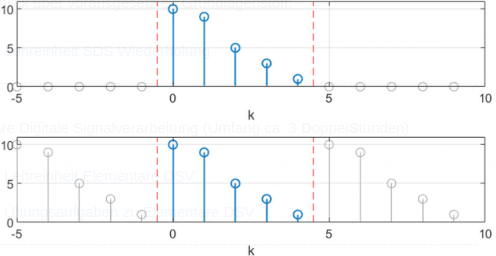
\includegraphics[width=.2\textwidth]{./img/x_k.png}
      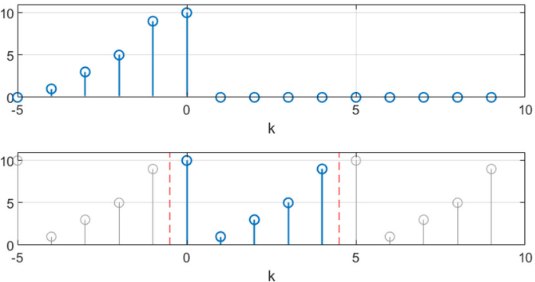
\includegraphics[width=.2\textwidth]{./img/x_mk.png}
  \end{center}
%%%%%%%%%%%%%%%%%%%%%%%%%%%%%%%%%%%%%%%%%%%%%%%%%%%%%%%%%%%%%%%%%%%%%%%%%%%%%%%%%%%%%%%%%%%%%%%%%%%%%%%%%%%%%%%
%%%%%%%%%%%%%%%%%%%%%%%%%%%%%%%%%%%%% DFT-Korrespondenzen %%%%%%%%%%%%%%%%%%%%%%%%%%%%%%%%%%%%%%%%%%%%%%%%%%%%%
\scriptsize
\begin{center}
\begin{tabular}{ | c | c | c | }
\cline{1-3}
        & Zeitbereich & Spektralbereich \\
\cline{1-3}
        Linearität & $a\cdot x_1(k)+ b\cdot x_2(k)$ & $a\cdot X_1(n) +b\cdot X_2(n)$ \\
\cline{1-3}
        Zeit-Verschiebung & $x([k\textcolor{red}{-}k_0]_{modN})$ & $e^{\textcolor{red}{-}j\frac{2\pi nk_0}{N}} X(n)$\\
\cline{1-3}
        Frequenz-Verschiebung & $e^{\textcolor{red}{-}j\frac{2\pi nk_0}{N}} x(k)$ & $X([n\textcolor{red}{+}k_0]_{modN})$ \\  
\cline{1-3}
        Spiegelung & $x([-k]_{modN})$ & $X([-n]_{modN})$ \\  
\cline{1-3}
        Konj.Kompl & $x^*(k)$& $X^*([-n]_{modN})$\\ 
\cline{1-3}
        Konj.Kompl.gespiegelt & $x^*([-k]_{modN})$& $X^*(n)$\\ 
\cline{1-3}
        Faltung & $x_1(k) \circledast x_2(k)$ & $X_1(n)X_2(n)$ \\  
\cline{1-3}
        Multiplikation & $x_1(k)x_2(k)$ & $\frac{1}{N} X_1(n) \circledast X_2(n)$ \\
\cline{1-3}
        gerade Symmetrie & $x_g(k)=\frac{x(k)+\tilde{x}(-k)}{2}$ & $X_g(n)=\frac{X(n)+X(-n)}{2}$ \\
\cline{1-3}
        ungerade Symmetrie & $x_u(k)=\frac{x(k)-\tilde{x}(-k)}{2}$ & $X_u(n)=\frac{X(n)-X(-n)}{2j}$ \\
\cline{1-3}
\end{tabular}
\end{center}
\normalsize
%%%%%%%%%%%%%%%%%%%%%%%%%%%%%%%%%%%%%%%%%%%%%%%%%%%%%%%%%%%%%%%%%%%%%%%%%%%%%%%%%%%%%%%%%%%%%%%%%%%%%%%%%%%%
%%%%%%%%%%%%%%%%%%%%%%%%%%%%%%%%%%%%% DFT-Korrespondenzen %%%%%%%%%%%%%%%%%%%%%%%%%%%%%%%%%%%%%%%%%%%%%%%%%%%%%
  \begin{center}
      \includegraphics[width=.35\textwidth]{./img/dtft.png}
  \end{center}
  \begin{center}
      \includegraphics[width=.35\textwidth]{./img/dft.png}
  \end{center}
%%%%%%%%%%%%%%%%%%%%%%%%%%%%%%%%%%%%%%%%%%%%%%%%%%%%%%%%%%%%%%%%%%%%%%%%%%%%%%%%%%%%%%%%%%%%%%%%%%%%%%%%%%%%
%%%%%%%%%%%%%%%%%%%%%%%%%%%%%%%%%%%%% z-Transformation %%%%%%%%%%%%%%%%%%%%%%%%%%%%%%%%%%%%%%%%%%%%%%%%%%%%%
  \subsection{z-Transformation}
  \begin{mdframed}[style=exercise]
    \begin{align}
        X(z) &=\sum_{k=-\infty}^{\infty} x(k)z^{-k} \ \ z=e^{s T_a}
    \end{align}
  \end{mdframed}
%%%%%%%%%%%%%%%%%%%%%%%%%%%%%%%%%%%%%%%%%%%%%%%%%%%%%%%%%%%%%%%%%%%%%%%%%%%%%%%%%%%%%%%%%%%%%%%%%%%%%%%%%%%%
%%%%%%%%%%%%%%%%%%%%%%%%%%%%%%%%%%%%% z-Korrespondenzen %%%%%%%%%%%%%%%%%%%%%%%%%%%%%%%%%%%%%%%%%%%%%%%%%%%%
  \begin{center}
      \includegraphics[width=.35\textwidth]{./img/z.png}
  \end{center}
%%%%%%%%%%%%%%%%%%%%%%%%%%%%%%%%%%%%%%%%%%%%%%%%%%%%%%%%%%%%%%%%%%%%%%%%%%%%%%%%%%%%%%%%%%%%%%%%%%%%%%%%%%%%
%%%%%%%%%%%%%%%%%%%%%%%%%%%%%%%%%%%%%%%%%% Faltung %%%%%%%%%%%%%%%%%%%%%%%%%%%%%%%%%%%%%%%%%%%%%%%%%%%%%%%%%
  \subsection{Faltung}
  \subsubsection{Lineare Faltung (\textbf{Octave:} conv)}
  \begin{mdframed}[style=exercise]
    \begin{align}
        g(k)*u(k) = \sum_{\nu =0}^{k} g(\nu) u(k-\nu)= \sum_{\nu =0}^{k} g(k-\nu) u(\nu)
    \end{align}
  \end{mdframed}
  \subsubsection{Zyklische Faltung (\textbf{Octave:} cconv)}
  $x_1(k)$ und $x_2(k)$ durch \textbf{Zero-Padding} auf $N = N_1 +N_2 -1$ 
\scriptsize
  \begin{mdframed}[style=exercise]
    \begin{align}
        x_1(k) \circledast x_2(k) = \sum_{\nu =0}^{N-1} x_1(\nu) x_2([k-\nu]_{modN})= \sum_{\nu =0}^{N-1}x_1([k-\nu]_{modN}) x_2(\nu)
    \end{align}
  \end{mdframed} 
  \subsubsection{Faltung in Matrixschreibweise}
  \textbf{ACHTUNG:} Auch hier gilt wieder $N_{y}=N_{1}+N_{2}-1$!
  \begin{center}
    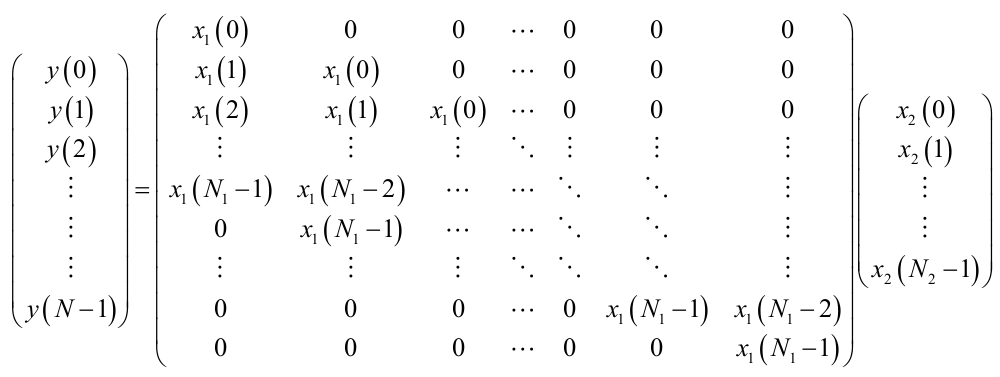
\includegraphics[width=.5\textwidth]{./img/Faltung_Matrixschreibweise.png}
\end{center}
\normalsize
%%%%%%%%%%%%%%%%%%%%%%%%%%%%%%%%%%%%%%%%%%%%%%%%%%%%%%%%%%%%%%%%%%%%%%%%%%%%%%%%%%%%%%%%%%%%%%%%%%%%%%%%%%%%
%%%%%%%%%%%%%%%%%%%%%%%%%%%%%%%%%%%%% Korrelation %%%%%%%%%%%%%%%%%%%%%%%%%%%%%%%%%%%%%%%%%%%%%%%%%%%%%%%%%%
  \subsection{Korrelation}
  $x_1(k) \in [0,N_1-1]$ und $x_2(k) \in [0,N_2-1]$ nicht kommutativ sondern an der y-Achse gespiegelt ($r_{x1x2}(\lambda)=r_{x2x1}(-\lambda)$).
  \begin{mdframed}[style=exercise]
    \begin{align}
        r_{x_1x_2}(\lambda) = \sum_{k=-\infty}^{\infty}x_1^*(k) x_2(k+\lambda)
    \end{align}
  \end{mdframed}
\textbf{Korrelation durch schnelle Faltung:}\\
1. Beide Signale Zero-Padding auf $N = N_1+N_2-1$\\
2. $x_1$ Spiegeln ($x_1^*(-\lambda)$)\\
3. Faltung ausführen
  \begin{mdframed}[style=exercise]
    \begin{align}
        r_{x_1x_2}(\lambda) = x_1^*(-\lambda)*x_2(\lambda)
    \end{align}
  \end{mdframed}
\begin{itemize}
    \item Nicht-Erwartungstreue Schätzung $\hat{\varphi}_{x1x2}$
    \item Erwartungstreue Schätzung $\hat{\varphi}_{x1x2}^{'}$
    \item Normierung auf $N = max(N_1,N_2)$
\end{itemize}
  \begin{mdframed}[style=exercise]
    \begin{align}
        \hat{\varphi}_{x_1x_2} &= \frac{1}{N} r_{x_1x_2}(\lambda)\\
        \hat{\varphi}_{x_1x_2}^{'} &= \frac{1}{N-\abs{\lambda}} r_{x_1x_2}(\lambda)
    \end{align}
  \end{mdframed}
Korrelationskoeffizient:
  \begin{center}
      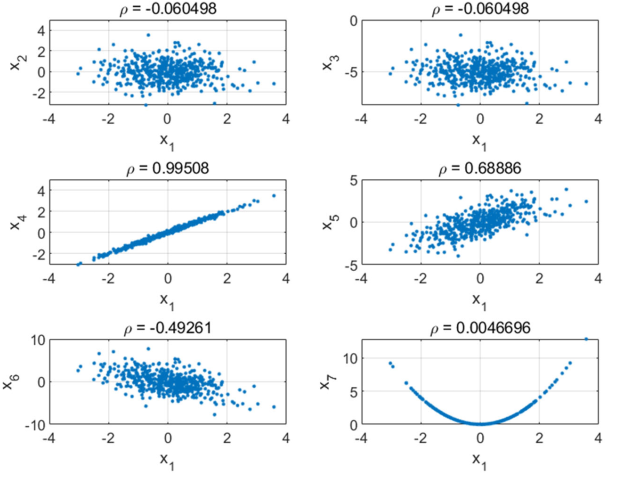
\includegraphics[width=.35\textwidth]{./img/korkoeff.png}
  \end{center}
%%%%%%%%%%%%%%%%%%%%%%%%%%%%%%%%%%%%%%%%%%%%%%%%%%%%%%%%%%%%%%%%%%%%%%%%%%%%%%%%%%%%%%%%%%%%%%%%%%%%%%%%%%
%%%%%%%%%%%%%%%%%%%%%%%%%%%%%%%%%%%%% Blocksignalverarbeitung %%%%%%%%%%%%%%%%%%%%%%%%%%%%%%%%%%%%%%%%%%%%
  \subsection{Blocksignalverarbeitung}
  Der $i$-te Block $x^{(i)}(k)$ der Länge $L$ mit Versch.abstand $D$ 
  wird als Multiplikation mit Fensterfunktion $w(k)$ beschrieben
  \begin{mdframed}[style=exercise]
    \begin{align}
        Allg.:
        x^{(i)}(k) = x(k+(i-1)D) \cdot w(k)\ \ k\in[0,L-1] 
    \end{align}
  \end{mdframed}
  Überlapp $D_\%$
  \begin{mdframed}[style=exercise]
    \begin{align}
        D_\% = \frac{L-D}{L}100\%
    \end{align}
  \end{mdframed}
% Overlapp-Add
  \subsubsection{Overlapp-Add Verfahren}
  Schnelle Faltung $g(k)*u(k)$ $N_u >> N_g$ 
  Aufteilung $u(k)$ nicht-überlappend (\textbf{nahtlos}) $\rightarrow D=L$ \\
  Zero-Padding $u^{(i)}(k)$ auf $N=L+N_g$ 
% Overlapp-Save
  \subsubsection{Overlapp-Save Verfahren}
  Schnelle Faltung $g(k)*u(k)$ $N_u >> N_g$ \\
  z.B Überlapp = $N_g-1 \rightarrow D=L-N_g+1$ \\
  \begin{mdframed}[style=exercise]
    \begin{align}
        u^{(i)}(k) = u(k+(i-1)D) \ \ k\in[0,L-1]
    \end{align}
  \end{mdframed}
%%%%%%%%%%%%%%%%%%%%%%%%%%%%%%%%%%%%%%%%%%%%%%%%%%%%%%%%%%%%%%%%%%%%%%%%%%%%%%%%%%%%%%%%%%%%%%%%%%%%%%%%%%
%%%%%%%%%%%%%%%%%%%%%%%%%%%%%%%%%%%%% Simultane Transformation %%%%%%%%%%%%%%%%%%%%%%%%%%%%%%%%%%%%%%%%%%%
  \subsection{Simultane Transformation}
  \begin{mdframed}[style=exercise]
    \begin{align}
        x_1(k) &= Re[y(k)] = \frac{1}{2}(y(k)+y^*(k))\\
        x_2(k) &= Im[y(k)] = \frac{1}{2j}(y(k)-y^*(k))\\
        x_1(k) &= x(2k)\\
        x_2(k) &= x(2k+1)\\
        y(k) &= x_1(k) +jx_2(k)
    \end{align}
  \end{mdframed}
  \begin{mdframed}[style=exercise]
    \begin{align}
        X_1(n) = \frac{1}{2}(Y(n)+Y^*([-n]_{modN}))\\
        X_2(n) = \frac{1}{2j}(Y(n)-Y^*([-n]_{modN}))
    \end{align}
  \end{mdframed}

%%%%%%%%%%%%%%%%%%%%%%%%%%%%%%%%%%%%%%%%%%%%%%%%%%%%%%%%%%%%%%%%%%%%%%%%%%%%%%%%%%%%%%%%%%%%%%%%%%%%%%%%%%
%%%%%%%%%%%%%%%%%%%%%%%%%%%%%%%%%%%%% Stochastische Prozesse %%%%%%%%%%%%%%%%%%%%%%%%%%%%%%%%%%%%%%%%%%%
\section{Stochastische Prozesse}
%%%%%%%%%%%%%%%%%%%%%%%%%%%%%%%%%%%%% Stochastische Variable %%%%%%%%%%%%%%%%%%%%%%%%%%%%%%%%%%%%%%%%%%%
\subsection{Wahrscheinlichkeitsdichtefunktion}
Wahrscheinlickkeit $P(x_u \leq x \leq x_o )$, dass $x \in [x_u,x_o]$ 
  \begin{mdframed}[style=exercise]
    \begin{align}
        P(x_u \leq x \leq x_o ) = \displaystyle\int_{x_u}^{x_o} f_x(\alpha) d\alpha \\
        bzw. \ \ F_x(\alpha) = \displaystyle\int_{-\infty}^{\alpha} f_x(u)du\\
        \displaystyle\int_{-\infty}^{\infty} f_x(u)du = 1
    \end{align}
  \end{mdframed}
Gaußverteilung (Normalverteilung)
  \begin{mdframed}[style=exercise]
    \begin{align}
        f_x(\alpha) = \frac{1}{\sigma_x \cdot \sqrt{2\pi}} \cdot e^{-\frac{1}{2} \cdot \left( \frac{\alpha - \mu_x}{\sigma_x}\right)^2}
    \end{align}
  \end{mdframed}
\subsection{Erwartungswert $\mu_x$, Varianz $\sigma_x^2$}
Formeln gelten nur für \textbf{stationäre} Zufallsvariablen bzw stochastische Prozesse
  \begin{mdframed}[style=exercise]
    \begin{align}
        \mu_x = E[x] = \displaystyle\int_{-\infty}^{\infty} \alpha f_x(\alpha) d\alpha = \displaystyle\sum_{\nu}^{} a_\nu P_\nu\\
        \sigma_x^2 = E[(x-\mu_x)^2] = E[x^2]-\mu_x^2  = \displaystyle\int_{-\infty}^{\infty} (\alpha-\mu_x)^2 \ f_x(\alpha) d\alpha
    \end{align}
  \end{mdframed}
Für 2 Stoch. unabh. Variablen $f_x(\alpha)$ und $f_y(\beta)$ \\
gilt bei $f_{xy}(\alpha,\beta) = f_x(\alpha)\cdot f_y(\beta)$:\\
  \begin{mdframed}[style=exercise]
    \begin{align}
        \mu_{xy} &= \mu_{x} + \mu_{y}\\
        \sigma_{xy}^2 &= \sigma_{x}^2 + \sigma_{y}^2
    \end{align}
  \end{mdframed}
\begin{minipage}{0.5\textwidth}  
Bei $f_{xy}(\alpha,\beta) = a\cdot f_x(\alpha)+ b\cdot f_y(\beta)$ gilt:\\
  \begin{mdframed}[style=exercise]
    \begin{align}
        \mu_{xy} = a\cdot \mu_{x} + b \cdot \mu_{y}\\
        \sigma_{xy} = E\{f_{xy}^{2}\}-\mu_{xy}^{2}=E\{(a\cdot f_x(\alpha)+ b\cdot f_y(\beta))^{2}\}
    \end{align}
  \end{mdframed}
\end{minipage}
% Für ein deterministisches Signal $x(k)$ gilt $\sigma_x^2=Var(x)=0$
% Falls $y(k) = x_1(k)x_2(k)$, dann gilt
%
%   \begin{mdframed}[style=exercise]
%     \begin{align}
%         \sigma_y^2 = (\sigma_{x_1}^2+\mu_{x_1}^2)(\sigma_{x_2}^2+\mu_{x_2}^2) 
%     \end{align}
%   \end{mdframed}
\subsection{Stationärer Stochastischer Prozess}
P. stationär, wenn seine \textcolor{red}{statistischen} Eigenschaften \textcolor{red}{zeitinvariant} sind \\
Einzelner stationärer Stochastischer Prozess:
  \begin{mdframed}[style=exercise]
    \begin{align}
        f_{x(k)}(\alpha) = f_{x(k+k_0)}(\alpha) = f_x(\alpha)
    \end{align}
  \end{mdframed}
Ein Prozess wird zu zwei verschiedene Zeitpunkte $k_1$ und $k_2$
  \begin{mdframed}[style=exercise]
    \begin{align}
        f_{x(k_1)x(k_2)}(\alpha) = f_{x(k_1+k_0)x(k_2+k_0)}(\alpha)
    \end{align}
  \end{mdframed}
Zwei Prozesse $x$ und $y$ wird zu zwei verschiedene Zeitpunkte $k_1$ und $k_2$
\begin{mdframed}[style=exercise]
    \begin{align}
        f_{x(k_1)y(k_2)}(\alpha) = f_{x(k_1+k_0)y(k_2+k_0)}(\alpha)
    \end{align}
  \end{mdframed}
Autokorrelations $\varphi_{xx}(\lambda)$ und Kreuzkorrelation $\varphi_{xy}(\lambda)$
\begin{mdframed}[style=exercise]
    \begin{align}
        \varphi_{xx}(\lambda) = E[x^*(k)x(k+\lambda)] \\
        \varphi_{xy}(\lambda) =E[x^*(k)y(k+\lambda)]
    \end{align}
  \end{mdframed}
Definition \textbf{schwache Stationarität}
\begin{itemize}
    \item $\mu_x = E[x(k)] = const.$
    \item $\varphi_{xx}(\lambda) = \varphi_{xx}(-\lambda)$ (= gerade Symmetrie)
    \item $\varphi_{xx}(0) \geq \abs{\varphi_{xx}(\lambda)}$ (max(Autokorr.) im Ursprung)
    \item $\varphi_{xx}(0) =E[\abs{x(k)}^2]$ (= mittlere Leistung)
    \item $\varphi_{xx}(0) = \sigma_x^2 + \abs{\mu_x}^2$
    \item aus Stationarität folgt \textbf{Unkorreliertheit}
\end{itemize}
%%%%%%%%%%%%%%%%%%%%%%%%%%%%%%%%%%%%%%%%%%%%%%%%%%%%%%%%%%%%%%%%%%%%%%%%%%%%%%%%%%%%%%%%%%%%%%%%%%%%%%%%%%
%%%%%%%%%%%%%%%%%%%%%%%%%%%%%%%%%%%%% Ergodizität %%%%%%%%%%%%%%%%%%%%%%%%%%%%%%%%%%%%%%%%%%%
\subsection{Ergodizität}
Scharmittelwert und Zeitmittelwert sind aquivalent\\
\scriptsize
\begin{center}
\begin{tabular}{|c|c|c|}
\cline{1-3}
        & Zeitmittelwert(Schätzung) & Scharmittelwert \\
\cline{1-3}
        lin. Mittelw $\mu_x$ & $\mu_x = \frac{1}{N}\sum_{k=0}^{N-1}x(k)$ & E[x(k)] \\
\cline{1-3}
        Varianz $\sigma_x^2$ & $\sigma_x^2 = \frac{1}{N}\sum_{k=0}^{N-1}\abs{x(k)-\mu_x}^2$ & $E[\abs{x(k)-\mu_x}^2]$ \\
\cline{1-3}
        AKorr. $\varphi_{xx}(\lambda)$ & $\frac{1}{N}\sum_{k=0}^{N-1} x^*(k)x(k+\lambda) $ & $E[x^*(k)x(k+\lambda)]$ \\
\cline{1-3}
        KKorr. $\varphi_{xy}(\lambda)$ & $\varphi_{xy}(\lambda)=\frac{1}{N}\sum_{k=0}^{N-1} x^*(k)y(k+\lambda) $ & $E[x^*(k)y(k+\lambda)]$ \\
\cline{1-3}
\end{tabular}
\end{center}
\normalsize
%%%%%%%%%%%%%%%%%%%%%%%%%%%%%%%%%%%%%%%%%%%%%%%%%%%%%%%%%%%%%%%%%%%%%%%%%%%%%%%%%%%%%%%%%%%%%%%%%%%%%%%%%%
%%%%%%%%%%%%%%%%%%%%%%%%%%%%%%%%%%%%% Leistungsdichtespektrum %%%%%%%%%%%%%%%%%%%%%%%%%%%%%%%%%%%%%%%%%%%%
\subsection{Leistungsdichtespektrum LDS}
LDS = DFT der Stochastischen Prozesse \\
Autoleistungsdichtespektrum  $\phi_{xx}(e^{j\Omega})$ und Kreuzeistungsdichtespektrum $\phi_{xy}(e^{j\Omega})$
  \begin{mdframed}[style=exercise]
    \begin{align}
        \phi_{xx}(e^{j\Omega}) &= \mathcal{F}\{ \varphi_{xx}(\lambda)\} \\
        \phi_{xx}(e^{j\Omega}) &= \sum_{\lambda=-\infty}^{\infty} \varphi_{xx}(\lambda) e^{-j\Omega\lambda} \\
        \varphi_{xx}(\lambda) &= \frac{1}{2\pi} \displaystyle\int_{-\pi}^{\pi} \phi_{xx}(e^{j\Omega})e^{j\Omega\lambda}d\Omega \\
        \phi_{xy}(e^{j\Omega}) &= \sum_{\lambda=-\infty}^{\infty} \varphi_{xy}(\lambda) e^{-j\Omega\lambda} \\
        \varphi_{xy}(\lambda) &= \frac{1}{2\pi} \displaystyle\int_{-\pi}^{\pi} \phi_{xy}(e^{j\Omega})e^{j\Omega\lambda}d\Omega \end{align}
  \end{mdframed}
Mittlere Leistung $\varphi_{xx}(0)$
  \begin{mdframed}[style=exercise]
    \begin{align}
        \varphi_{xx}(0) = \frac{1}{2\pi} \displaystyle\int_{-\pi}^{\pi} \phi_{xx}(e^{j\Omega})d\Omega  = \frac{\phi_{xx}(e^{j\Omega})}{2\pi}
    \end{align}
  \end{mdframed}
Weißes Rauschen (Mittelwertfrei) 
  \begin{mdframed}[style=exercise]
    \begin{align}
        \phi_{xx}(e^{j\Omega}) = \phi_0\\
        \varphi_{xx}(0) = \phi_0 \gamma_0(\lambda)
    \end{align}
  \end{mdframed}
%%%%%%%%%%%%%%%%%%%%%%%%%%%%%%%%%%%%%%%%%%%%%%%%%%%%%%%%%%%%%%%%%%%%%%%%%%%%%%%%%%%%%%%%%%%%%%%%%%%%%%%%%%
%%%%%%%%%%%%%%%%%%%%%%%%%%%%%%%%%%%%% LTI-Systeme %%%%%%%%%%%%%%%%%%%%%%%%%%%%%%%%%%%%%%%%%%%%%%%%%%%%%%%%
\subsection{LTI-Systeme}
  \begin{center}
      \includegraphics[width=.5\textwidth]{./img/lti.png}
  \end{center}
Mit konst. Mittelwerten $E[u(k-\nu)]=\mu_x$ und $E[y(k)]=\mu_y$
  \begin{mdframed}[style=exercise]
    \begin{align}
        \mu_y = \mu_u \sum_{\nu=-\infty}^{\infty} h(\nu) = \mu_u H(e^{j0})
    \end{align}
  \end{mdframed}
\textbf{Zusätzliche Beziehungen:}
  \begin{mdframed}[style=exercise]
    \begin{align}
        \varphi_{uy}(\lambda) &= h(\lambda)*\varphi_{uu}(\lambda) \\
        \varphi_{yu}(\lambda) &= h(-\lambda)^**\varphi_{uu}(\lambda) \\
        \varphi_{yy}(\lambda) &= h(\lambda)*\varphi_{yu}(\lambda) = h^*(-\lambda)*\varphi_{uy}(\lambda) \\
        \varphi_{yy}(\lambda) &= h^*(-\lambda)*h(\lambda)*\varphi_{uu}(\lambda)
    \end{align}
  \end{mdframed}

\begin{mdframed}[style=exercise]
    \begin{align}
      \phi_{uy}(e^{j\Omega}) = H(e^{j\Omega})\phi_{uu}(e^{j\Omega})\\
      \phi_{yu}(e^{j\Omega}) = H^*(e^{j\Omega})\phi_{uu}(e^{j\Omega})\\
      \phi_{yy}(e^{j\Omega}) = H^*(e^{j\Omega})H(e^{j\Omega})\phi_{uu}(e^{j\Omega}) =\abs{H(e^{j\Omega})}^2 \phi_{uu}(e^{j\Omega})
    \end{align}
\end{mdframed}

  
%%%%%%%%%%%%%%%%%%%%%%%%%%%%%%%%%%%%%%%%%%%%%%%%%%%%%%%%%%%%%%%%%%%%%%%%%%%%%%%%%%%%%%%%%%%%%%%%%%%%%%%%%%
%%%%%%%%%%%%%%%%%%%%%%%%%%%%%%%%%%%%% Spektralschätzung %%%%%%%%%%%%%%%%%%%%%%%%%%%%%%%%%%%%%%%%%%%%%%%%%%%%%%%%
  \section{Spektralschätzung}
  \subsection{Spektralschätzung mit FFT}
  Umrechnung $n \leftrightarrow f$
  \begin{mdframed}[style=exercise]
    \begin{align}
        f_n = n\frac{f_A}{N}
    \end{align}
  \end{mdframed}
  Umrechnung $\Omega \leftrightarrow n$
  \begin{mdframed}[style=exercise]
    \begin{align}
        \Omega_n = 2\pi\frac{n}{N} = \omega T_a
    \end{align}
  \end{mdframed}
  Umrechnung $\omega \leftrightarrow n$
  \begin{mdframed}[style=exercise]
    \begin{align}
        \omega_n = 2\pi f_A\frac{n}{N} 
    \end{align}
  \end{mdframed}
    \begin{center}
    \begin{tabular}{c c}
        Spektrum & Zeitbereich \\
        $n=0$ & Konstante $x(0)=\frac{1}{N}X(0)$\\
        $n=\tilde{n}$ & $ x_{\tilde{n}}(k)=\frac{1}{N}( X(\tilde{n})e^{-j\frac{2\pi k\tilde{n}}{N}}+X(N-\tilde{n})e^{-j\frac{2\pi k(N-\tilde{n})}{N}})$\\
        $n=\frac{N}{2}$ & $e^{jk\pi} = (-1)^k$\\
    \end{tabular}
    \end{center}
%%%%%%%%%%%%%%%%%%%%%%%%%%%%%%%%%%%%%%%%%%%%%%%%%%%%%%%%%%%%%%%%%%%%%%%%%%%%%%%%%%%%%%%%%%%%%%%%%%%%%%%%%%
%%%%%%%%%%%%%%%%%%%%%%%%%%%%%%%%%%%%% Leck-Effekt %%%%%%%%%%%%%%%%%%%%%%%%%%%%%%%%%%%%%%%%%%%%%%%%%%%%%%%%
\subsection{Leck-Effekt}
Kein Ganzzahliges Vielfaches fällt in das Beobachtungsfenster $w(k)$.\\
Bsp: Sinus $x(t) = sin(w_0t)\cdot w(t)$ mit $w(t)=rect(\frac{t-T/2}{T})$
  \begin{mdframed}[style=exercise]
        $x_w(k) = x(k)w(k) \laplace \  X_w(n) = X(n)*W(n) \\
        sin(w_0t) \fourier j\pi(\delta_0(w+w_0)-\delta_0(w-w_0))\\
        rect(\frac{t-T/2}{T}) \fourier Tsi(w\frac{T}{2})e^{-jw\frac{T}{2}}\\
        X(jw)=\frac{2}{2\pi}[j\pi(\delta_0(w+w_0)-\delta_0(w+w_0))]*si(w\frac{T}{2})e^{-jw\frac{T}{2}}]\\
        X(jw)=j\frac{T}{2}[si((w+w_0)\frac{T}{2})e^{-j(w+w_0)\frac{T}{2}} - si((w-w_0)\frac{T}{2})e^{-j(w-w_0)\frac{T}{2}}]$
  \end{mdframed}
%%%%%%%%%%%%%%%%%%%%%%%%%%%%%%%%%%%%%%%%%%%%%%%%%%%%%%%%%%%%%%%%%%%%%%%%%%%%%%%%%%%%%%%%%%%%%%%%%%%%%%%%%%
%%%%%%%%%%%%%%%%%%%%%%%%%%%%%%%%%%%%% Fensterfunktionen %%%%%%%%%%%%%%%%%%%%%%%%%%%%%%%%%%%%%%%%%%%%%%%%%%%%%%%%
\subsection{Zeitfenster}
  \begin{center}
      \includegraphics[width=.16\textwidth]{./img/rect.png}
      \includegraphics[width=.15\textwidth]{./img/hamming.png}
      \includegraphics[width=.16\textwidth]{./img/hann.png}
  \end{center}
  Rechteck um bei k=0 beginnend (um $\frac{N}{2}$ verschoben)
  \begin{mdframed}[style=exercise]
    \begin{align}
        rect(k-\frac{N}{2}) \fourier \frac{sin(N\frac{\Omega}{2})}{sin(\frac{\Omega}{2})} e^{-j\Omega\frac{N-1}{2}}
    \end{align}
  \end{mdframed}
  \begin{itemize}
    \item Breite der Hauptkeule $\Omega_B = \frac{4\pi}{N}$
    \item Höhe der Hauptkeule $A_B = N$
    \item Nullstellen $\Omega_{0\nu} = \frac{2\pi}{N}\nu \ \ \nu \in\mathbb{Z} \textbackslash\{0\}$
  \end{itemize}
\subsection{Zero-Padding}
Zero-Padding = Annäherung an die DTFT $\rightarrow$ feinere Spektrumauflösung Energiegehalt $E = E_{ZP}$ \\
%%%%%%%%%%%%%%%%%%%%%%%%%%%%%%%%%%%%%%%%%%%%%%%%%%%%%%%%%%%%%%%%%%%%%%%%%%%%%%%%%%%%%%%%%%%%%%%%%%%%%%%%%%
%%%%%%%%%%%%%%%%%%%%%%%%%%%%%%%%%%%%% Spektral Stoch. Prozesse %%%%%%%%%%%%%%%%%%%%%%%%%%%%%%%%%%%%%%%%%%%%%%%%%%%%%%%%

\subsection{Spektralschätzung Stoch. Prozesse}
Periodogramm
  \begin{mdframed}[style=exercise]
    \begin{align}
        \hat{\phi}_{Per} = \frac{1}{N}\abs{X(n)}^2
    \end{align}
  \end{mdframed}
Mittlere Leistung P mittels Periodogramm
  \begin{mdframed}[style=exercise]
    \begin{align}
        P = \frac{1}{N}\sum_{n=0}^{N-1} \hat{\phi}_{Per} = \frac{1}{N^2}\sum_{n=0}^{N-1} \abs{X(n)}^2
    \end{align}
  \end{mdframed}
Falls nur Spektrum von $n\in [0,N/2]$ gegeben (N ist gerade)
  \begin{mdframed}[style=exercise]
    \begin{align}
        P = \frac{1}{N}( \hat{\phi}_{Per}(0) + 2 sum_{n=0}^{N/2-1} \hat{\phi}_{Per} + \hat{\phi}_{Per}(\frac{N}{2})) \\
        P = \frac{1}{N^2}( \abs{X(0)}^2 + 2 \sum_{n=0}^{N/2-1} \abs{X(n)}^2 + \abs{X(N/2)}^2) 
    \end{align}
  \end{mdframed}
Falls nur best. Frequenzintervall $P\in [f_u,f_0] \rightarrow [n_1,n_2]$\\ 
$n_{1} > 0$ und $n_{2} < N/2$ (N ist gerade)
  \begin{mdframed}[style=exercise]
    \begin{align}
        P = \frac{2}{N}\sum_{n=n_1}^{n_2} \hat{\phi}_{Per} = \frac{2}{N^2}\sum_{n=n_1}^{n_2} \abs{X(n)}^2
    \end{align}
  \end{mdframed}
Auch hier tritt Leck-Effekt auf $\rightarrow$ Minderung mit Fensterfunktion w(t) 
ABER: Verlust von Energie => Modifikation d. Schätzung mit Korrekturfaktor $U$ (hängt von w(t) ab)
Spezialfall: w(t) = rect(t) => U = 1 
  \begin{mdframed}[style=exercise]
    \begin{align}
        \hat{\phi}_{Per,m} = \frac{1}{NU}\abs{X_m(n)}^2\\
        U = \frac{1}{N}\sum_{k=0}^{N-1} \abs{w(t)}^2 
    \end{align}
  \end{mdframed}
%%%%%%%%%%%%%%%%%%%%%%%%%%%%%%%%%%%%%%%%%%%%%%%%%%%%%%%%%%%%%%%%%%%%%%%%%%%%%%%%%%%%%%%%%%%%%%%%%%%%%%%%%%
%%%%%%%%%%%%%%%%%%%%%%%%%%%%%%%%%%%%% Weißes Rauschen %%%%%%%%%%%%%%%%%%%%%%%%%%%%%%%%%%%%%%%%%%%%%%%%%%%%%%%%
\subsubsection{Weißes Rauschen}
LDS ist Konstante $\phi_{xx,WR}(n) = \phi_{xx,WR} = const.$
  \begin{mdframed}[style=exercise]
    \begin{align}
        P = \frac{1}{N} \sum_{n=0}^{N-1} \phi_{xx,WR}(n) = \phi_{xx,WR}
    \end{align}
  \end{mdframed}
%%%%%%%%%%%%%%%%%%%%%%%%%%%%%%%%%%%%%%%%%%%%%%%%%%%%%%%%%%%%%%%%%%%%%%%%%%%%%%%%%%%%%%%%%%%%%%%%%%%%%%%%%%
%%%%%%%%%%%%%%%%%%%%%%%%%%%%%%%%%%%%% Welch-Methode %%%%%%%%%%%%%%%%%%%%%%%%%%%%%%%%%%%%%%%%%%%%%%%%%%%%%%%%
\subsection{Welch-Methode}
Zerlegung von x(k) der Länge N in K Sequenzen $x^{(i)}(k)$ der Länge L. 
Die Startzeitpunkte liegen im Abstand D \\
Es gilt $N=L+D(K-1)$
  \begin{mdframed}[style=exercise]
    \begin{align}
        x^{(i)}(k) = x(k+iD) \ \ k\in[0,L-1] 
    \end{align}
  \end{mdframed}
z.B Fensterung + Zero-Padding $\tilde{L} = L + L_{ZP}$
  \begin{mdframed}[style=exercise]
    \begin{align}
        \hat{\phi}_{Per}^{(i)}(n) = \frac{1}{LU}\abs{X^{(i)}(n)}^2\\
        U = \frac{1}{L}\sum_{k=0}^{N-1} \abs{w(t)}^2 
    \end{align}
  \end{mdframed}
Das LDS ergiebt sich aus \textcolor{red}{Mittelung} aller K Periodogramme
  \begin{mdframed}[style=exercise]
    \begin{align}
        \hat{\phi}_{W}(n) = \frac{1}{K}\sum_{i=0}^{K-1} \hat{\phi}^{(i)}(n) \\
        P = \frac{1}{\tilde{L}}\sum_{n=0}^{\tilde{L}-1}\hat{\phi}_{W}(n)
    \end{align}
  \end{mdframed}
$K\uparrow$ => Varianz d. Schätzung$\downarrow$ => Qualität $\uparrow$\\
$L\downarrow$ => Frequenzauflösung$\downarrow$ \\
$D\downarrow$ => Überlapp$\uparrow$ => K$\uparrow$ => Rechenaufwand$\uparrow$
%%%%%%%%%%%%%%%%%%%%%%%%%%%%%%%%%%%%%%%%%%%%%%%%%%%%%%%%%%%%%%%%%%%%%%%%%%%%%%%%%%%%%%%%%%%%%%%%%%%%%%%%%%
%%%%%%%%%%%%%%%%%%%%%%%%%%%%%%%%%%%%% Digitale-Filter%%%%%%%%%%%%%%%%%%%%%%%%%%%%%%%%%%%%%%%%%%%%%%%%%%%%%%%%
\section{Digitale-Filter}
  \begin{mdframed}[style=exercise]
    \begin{align}
        H(z)=\frac{Y(z)}{U(z)}=\frac{\grqq{}Ausgangssignal\grqq{}}{\grqq{}Eingangssignal\grqq{}}\\
        H(z)=\frac{Y(z)}{U(z)}= \frac{\sum_{\mu=0}^{m} b_\mu z^{-\mu}}{\sum_{\nu=0}^{n} a_\nu z^{-\nu}}
    \end{align}
  \end{mdframed}

\subsection{Anmerkung LTI-Systeme:}
\begin{itemize}
    \item \textbf{Allgemein: }
    	\begin{itemize}
    	\item $z^{-1}$ entspricht Verzögerung um einen Abtastwert
    	\item z-Trans. = Laplace-Trans. für abgetastete Signale
    	\item $z = e^{j\cdot\Omega}=e^{(\delta + j \cdot \omega)\cdot T_a}$
    	\end{itemize}
    \item \textbf{Besonderheiten: }
    	\begin{itemize}
    	\item Bandbreite ist bei TP $\Delta \Omega = 2\cdot\Omega_{3dB}$ 
    	\item \textbf{Minimalphasigkeit: } NST \textbf{ausschließlich} mit negativem Realwert
    	\end{itemize}
    \item \textbf{Ordnung des Systems: } Maximum des Polynomgrades von m \& n
    \item \textbf{Stabilität: }
    	\begin{itemize}
	\item \textbf{Asympthotisch:} \textbf{alle} Beträge $\abs{b_{v}}<1$
	\item \textbf{Grenzstabil:} einfacher Pol mit $\abs{b_{v}}=1$
	\item \textbf{Instabil:} mindestens ein Betrag $\abs{b_{v}}>1$\\
	\textbf{ODER} doppelter Pol mit $\abs{b_{v}}=1$
	\end{itemize}	
    \item \textbf{Realisierbarkeit: }
    	\begin{itemize}
    	\item Realisierbar wenn \textbf{kausal UND stabil}
    	\item \textbf{Kausal: Polynomgrad $n \geq m$}\\
    	(\textbf{NICHT} von \textbf{zukünftigen} Werten abhängig)
    	\end{itemize}
\end{itemize}  

\subsection{Pol-Nullstellen-Diagramm:}
Darstellung Linearfaktoren für n=2
  \begin{mdframed}[style=exercise]
    \begin{align}
        H(z)=\frac{b_0(z-z_{01})(z-z_{02})}{a_0(z-z_{\infty 1})(z-z_{\infty 2})}
    \end{align}
  \end{mdframed}

\begin{itemize}
    \item Pole verstärkt Amplitudengang
    \item Nullstelle dämpft Amplitudengang
    \item Pole und Nullstellen treten immer \textbf{konj. komplex} auf
\end{itemize}
\begin{itemize}
    \item $(e^{j\Omega}-z_{01}) = D_{01}e^{j\phi_{01}}$ und $(e^{j\Omega}-z_{02}) = D_{02}e^{j\phi_{02}}$
    \item $(e^{j\Omega}-z_{\infty 1}) = D_{\infty 1}e^{j\phi_{01}}$ und $(e^{j\Omega}-z_{01}) = D_{\infty 2}e^{j\phi_{\infty 2}}$
\end{itemize}
  \begin{center}
      \includegraphics[width=.35\textwidth]{./img/ehk.png}
  \end{center}
\begin{itemize}
    \item \textbf{Amplitudengang: } $\abs{H(e^{j\Omega})}=\abs{\frac{b_0}{a_0}} \abs{ \frac{D_{01}D_{02}}{D_{\infty 1}D_{\infty 2}}}$
    \item \textbf{Phasengang: }\\
    $arg({H(e^{j\Omega})})=arg(\frac{b_0}{a_0}) +\phi_{01} +\phi_{02}-\phi_{\infty 1}-\phi_{\infty 2}$
\end{itemize}

\subsection{Besonderheiten: }
\begin{itemize}
    \item \textbf{Umrechnung Frequenz in Winkel:} $\varphi = \frac{2\cdot\pi\cdot f_{n}}{f_{Abtast}}$
    \item Auf Einheitskreis wird (gegen \textbf{Urzeigersinn})\\
    von 0 Hz (0°) bis $f_{Abtast}$ (360°) gelaufen
    \item \textbf{Skalierung der Pol- / Nullstellen: } \\
    Substitution von $N(z)$ durch $N(\frac{z}{c})$\\
    $N(z)=\sum_{\mu=0}^{m} b_\mu z^{-\mu}$ -> $N(\frac{z}{c})=\sum_{\mu=0}^{m} b_\mu (\frac{z}{c})^{-\mu}$
    \item\textbf{Hinweis Gruppenlaufzeit: } Sprünge der Phase beeinträchtigen die Gruppenlaufzeit nicht\\
    $\rightarrow$ Phasensprünge für Ableitung ignorieren!
\end{itemize}
 
%%%%%%%%%%%%%%%%%%%%%%%%%%%%%%%%%%%%%%%%%%%%%%%%%%%%%%%%%%%%%%%%%%%%%%%%%%%%%%%%%%%%%%%%%%%%%%%%%%%%%%%%%%
%%%%%%%%%%%%%%%%%%%%%%%%%%%%%%%%%%%%% Rekursiver Glätter %%%%%%%%%%%%%%%%%%%%%%%%%%%%%%%%%%%%%%%%%%%%%%%%%%%%%%%
\subsection{Rekursiver Glätter}
Vergangenheitswert y(k-1) wird mit Faktor $a\in [0,1]$
  \begin{mdframed}[style=exercise]
    \begin{align}
        y(k) &= ay(k-1)+(1-a)u(k) \\
        h(k) &= (1-a)\cdot a^{k} \cdot \sigma(k)\\
        H(z) &=\frac{1-a}{1-az^{-1}}=\frac{(1-a)z}{z-a}
    \end{align}
  \end{mdframed}
Vom Verhalten entspricht er einem Tiefpass 1.Ordnung mit Grenzfrequenz $\Omega_g$ (a lässt sich aus $\Omega_g$ berechnen)
  \begin{mdframed}[style=exercise]
    \begin{align}
        \Omega_g = 2\pi\frac{f_g}{f_A}= arccos(\frac{a^{2}-4\cdot a+1}{-2\cdot a})\\
        \abs{H(\Omega)}= \frac{1-a}{\sqrt{1-2\cdot a\cdot cos(\Omega)+a^{2}}}
        H(e^{j\Omega}) =\frac{1-a}{1-ae^{-j\Omega}}\\
        a = 2-cos(\Omega_g)-\sqrt{(2-cos(\Omega_g))^2-1}
    \end{align}
  \end{mdframed}
%%%%%%%%%%%%%%%%%%%%%%%%%%%%%%%%%%%%% Mittelwert %%%%%%%%%%%%%%%%%%%%%%%%%%%%%%%%%%%%%%%%%%%%%%%%%%%%%%%%
\subsection{Arithmetischer Mittelwert Glätter}
  \begin{mdframed}[style=exercise]
    \begin{align}
        y(k)&=\frac{1}{N}\sum_{\nu=0}^{N-1} u(k-\nu)\\
        H(z)&=\frac{1}{N}\sum_{\nu=0}^{N-1} z^{-\nu} = \frac{1}{N}\frac{z^{-N}-1}{z^{-1}-1}
    \end{align}
  \end{mdframed}
%%%%%%%%%%%%%%%%%%%%%%%%%%%%%%%%%%%%% Notch-Filter %%%%%%%%%%%%%%%%%%%%%%%%%%%%%%%%%%%%%%%%%%%%%%%%%%%%%%%%
\subsection{Notch-Filter}
  \begin{mdframed}[style=exercise]
    \begin{align}
        H(z)=\frac{(z-e^{j\Omega_0})(z-e^{-j\Omega_0})}{(z-r_{\infty}e^{j\Omega_0})(z-r_{\infty}e^{-j\Omega_0})}
    \end{align}
  \end{mdframed}
Vorgabe Kerbe bei Frequenz $f_N$ und -3dB Breite $\Delta f$ und gegebener Abtastfrequenz $f_A$
  \begin{mdframed}[style=exercise]
    \begin{align}
        \Omega_0=\frac{2\pi f_N}{f_A}\\
        \Delta\Omega=\frac{2\pi\Delta f}{f_A}
    \end{align}
  \end{mdframed}
Einsetzen in Übertragungsfunktion H(z), Kerbentiefe $+A_B[dB]$
  \begin{mdframed}[style=exercise]
    \begin{align}
        H(z)=b\frac{1-2cos(\Omega_0)z^{-1}+z^{-2}}{1-2bcos(\Omega_0)z^{-1}+(2b-1)z^{-2}}\\
        b=\frac{1}{1+\frac{\sqrt{1-G_B^2}}{G_B}tan(\frac{\Delta\Omega}{2})} \ mit \ G_B=10^{\frac{-A_B}{20}}
    \end{align}
  \end{mdframed}
%%%%%%%%%%%%%%%%%%%%%%%%%%%%%%%%%%%%% Kammfilter %%%%%%%%%%%%%%%%%%%%%%%%%%%%%%%%%%%%%%%%%%%%%%%%%%%%%%%%
\subsection{Kammfilter}
Zu jeder Nullstelle $z_{0n}$ einen Pol $z_{\infty n}$ im Radius $r_\infty<1$ plazieren.\\ 
p = Ordnung, (K) = Kerbenbildend, (R) = Resonanzbildend, n = 0..(p-1)
  \begin{mdframed}[style=exercise]
    \begin{align}
        z_{0n}^{(K)} &= e^{j\frac{2\pi n}{p}} \\
        z_{\infty n}^{(K)} &= r_\infty e^{j\frac{2\pi n}{p}}\\
        z_{0n}^{(R)} &= e^{j\frac{(\pi + 2\pi n)}{p}}\\
        z_{\infty n}^{(R)} &= r_\infty e^{j\frac{(2\pi n)}{p}}
    \end{align}
  \end{mdframed}
\subsubsection{Kerbenbildend Kammfilter $H_{(K)}(z)$}
Dimensionierung $b$, sodass zwischen Kerben $0dB(=1)$
  \begin{mdframed}[style=exercise]
    \begin{align}
        H_{(K)}(z)=\frac{1+r_\infty ^p}{2}\cdot \frac{1-z^{-p}}{1-r_\infty^p z^{-p}}
    \end{align}
  \end{mdframed}
\subsubsection{Resonanzbildender Kammfilter $H_{(R)}(z)$}
Dimensionierung $b$, sodass zwischen Kerben $0dB(=1)$
  \begin{mdframed}[style=exercise]
    \begin{align}
        H_{(R)}(z)= \frac{1-r_\infty ^p}{2}\cdot \frac{1+z^{-p}}{1-r_\infty^p z^{-p}}
    \end{align}
  \end{mdframed}
%%%%%%%%%%%%%%%%%%%%%%%%%%%%%%%%%%%%% Goertzel-Algorithmus %%%%%%%%%%%%%%%%%%%%%%%%%%%%%%%%%%%%%%%%%%%%%%%%%%%%%%%%
\subsection{Goertzel-Algorithmus}
Bestimmung eines einzelnen DFT-Spektralwert X(n). Gleicher Rechenaufwand wie FFT aber Blocklänge N muss keine 2er Potenz sein. $\tilde{x}(k)=[x(0..N-1) \ 0]$ (N-ter Wert 0 setzen)
  \begin{mdframed}[style=exercise]
    \begin{align}
        n_0 = \frac{f_0}{f_A}N\\
        X(n_0)= y(k)=x(k)*h(k)|_{k=N}\\
        X(n_0)=y_n(k)=\sum_{\nu=0}^{k}\tilde{x}(\nu)e^{j\frac{2\pi}{N}(k-\nu)n}\\
        h(k)=(e^{\frac{j\cdot 2\cdot\pi\cdot n}{N}})^{k}\cdot\sigma(k)\\
        n = -j\cdot\frac{N}{2\cdot\pi}\cdot ln(h(1)) \rightarrow f_{Goertzel}=\frac{f_{Abtast}}{N}\cdot n
    \end{align}
  \end{mdframed}
%%%%%%%%%%%%%%%%%%%%%%%%%%%%%%%%%%%%% IIR-Filter %%%%%%%%%%%%%%%%%%%%%%%%%%%%%(%%%%%%%%%%%%%%%%%%%%%%%%%%%
\subsection{IIR-Filter}
\begin{itemize}
  \item \textbf{Vorteile: }
    \begin{itemize}
     \item geringere Filterordnung bei vergl. FIR-Filter
     \item Entwurfswerkzeuge aus analoger Welt nutzbar
     \end{itemize}
  \item \textbf{Nachteile: }
    \begin{itemize}
    \item NICHT linearphasig
    \item Anfälligkeit gegen Wortlängeneffekte 
    \item Instabilität möglich
    \end{itemize}
\end{itemize}
  \begin{mdframed}[style=exercise]
    \begin{align}
        H(z)=\frac{Y(z)}{U(z)}= \frac{\sum_{\mu=0}^{m} b_\mu z^{-\mu}}{\sum_{\nu=0}^{n} a_\nu z^{-\nu}}\\
        \sum_{\nu=0}^{n}a_{\nu}\cdot y(k-v) = \sum_{\mu=0}^{m}b_{\mu}\cdot u(k-\mu)
    \end{align}
  \end{mdframed}
Gruppenlaufzeit $\tau$ = Verzögerungszeit des Systems aufgelöst nach Frequenzen
  \begin{mdframed}[style=exercise]
    \begin{align}
        \tau = -\frac{d}{df}\varphi
    \end{align}
  \end{mdframed}
\subsubsection{IIR-Entwurfsmethoden}
  \begin{center}
      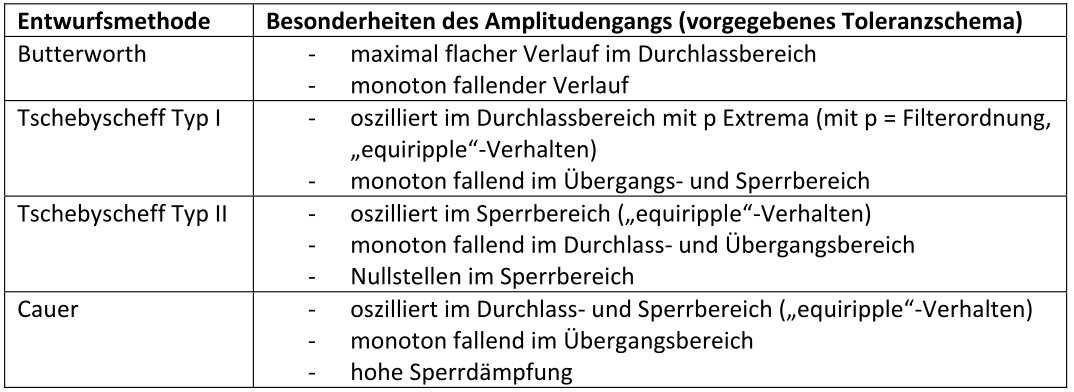
\includegraphics[width=.5\textwidth]{./img/entwurf.png}
  \end{center}

\textbf{Grundtypen von IIR-Filtern:}\\
(\textbf{Achtung: } Amplitudengang ist hier linear angegeben!)
\begin{center}
      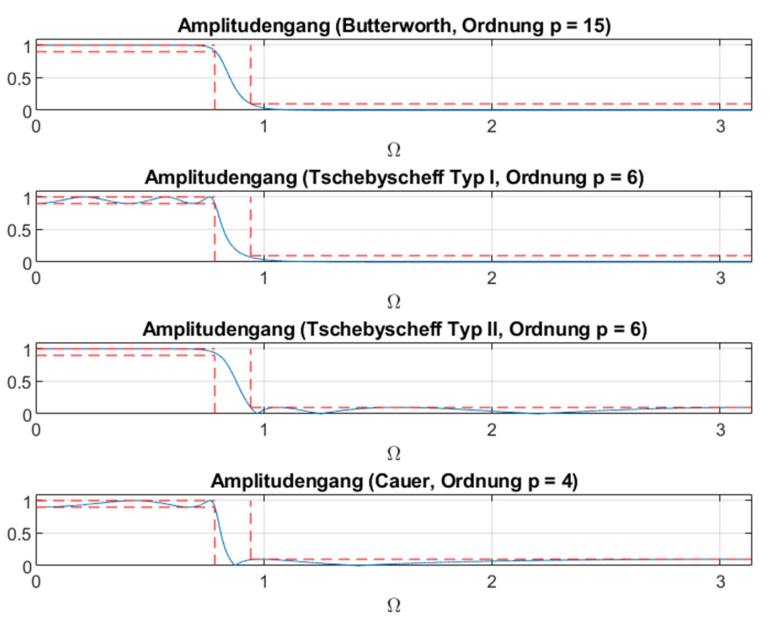
\includegraphics[width=0.50\textwidth]{./img/IIR_Filtertypen_Amplitudengang.png}
      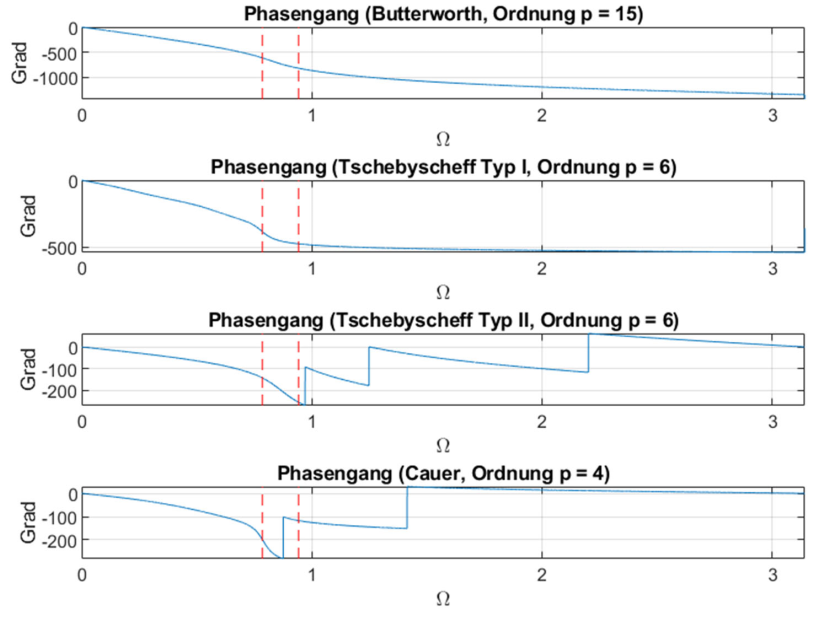
\includegraphics[width=0.50\textwidth]{./img/IIR_Filtertypen_Phasengang.png}
      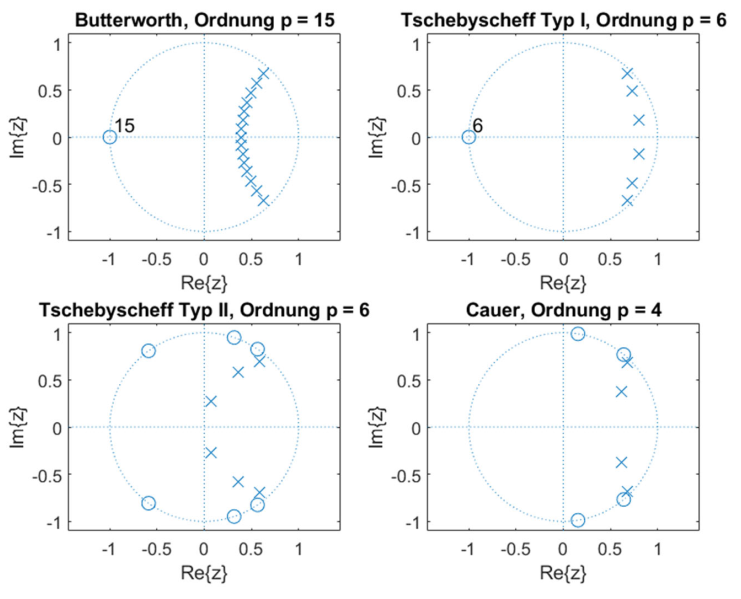
\includegraphics[width=0.50\textwidth]{./img/IIR_Filtertypen_Pol_NST.png}
\end{center}
%%%%%%%%%%%%%%%%%%%%%%%%%%%%%%%%%%%%% FIR-Filter %%%%%%%%%%%%%%%%%%%%%%%%%%%%%%%%%%%%%%%%%%%%%%%%%%%%%%%%
\begin{minipage}{0.5\textwidth}  
\subsection{FIR-Filter}
\begin{itemize}
  \item \textbf{Besonderheiten: }
       \begin{itemize}
       \item \textbf{nichtrekursiver} Filter mit \textbf{Grad m}
       \item m-facher Pol im Ursprung 
       \item Einsatz in adaptiven Systemen 
       \item Impulsantwort entspricht\\
       den b-Koeffizienten in $H(z)$
       \end{itemize}
  \item \textbf{Vorteile: }
    \begin{itemize}
     \item Linearphasigkeit \textbf{MÖGLICH}
     \item \textbf{IMMER} stabil
     \item endlich Ein- \& Ausschwingzeiten
     \end{itemize}
  \item \textbf{Nachteile: }
    \begin{itemize}
    \item große Filterordnung wenn hohe Sperrdämpfung / \\
    steile Filterflanken gefordert sind
    \item kann mit analogen Bauteilen \\
    NICHT realisiert werden
    \end{itemize}
\end{itemize}

  \begin{mdframed}[style=exercise]
    \begin{align}
        H(z)&=\frac{Y(z)}{U(z)}= \sum_{\mu=0}^{m} b_\mu z^{-\mu} \\
        H(z)&=\frac{b_0\Pi_{\mu=1}^{m}(z-z_{0\mu})}{z^m}\\
        h(k)&= b_k \ \ k\in[0,m] 
    \end{align}
  \end{mdframed}
\end{minipage}  
\begin{minipage}{0.5\textwidth} 
Gewollte Eigenschaft: \textbf{\textcolor{red}{lineare Phase}}
  \begin{mdframed}[style=exercise]
    \begin{align}
        \tau_{Gruppe} = -\frac{d}{d\Omega} arg(H(e^{j\Omega})) = const.
    \end{align}
  \end{mdframed}
Linearphasigkeit gilt wenn Nullstellen von H(z):
\begin{itemize}
    \item auf Einheitskreis
    \item \textbf{ODER} in am Einheitskreis gespiegelten Paaren\\
    ($z_{01}$ und $\frac{1}{z^*_{01}})$
\end{itemize}
auftreten.
  \begin{center}
      \includegraphics[width=0.8\textwidth]{./img/fir.png}
  \end{center}
Für linearphasige FIR-Filter der Ordnung p gilt\\
für Impulsantwort h(k):
\begin{itemize}
    \item $h(k)= h(p-k)$ (gerade Symmetrie) 
    \item $h(k)= -h(p-k)$ (ungerade Symmetrie)\\
\end{itemize}
\end{minipage}
\begin{minipage}{0.5\textwidth} 
\subsubsection{Grundtypen von FIR-Filtern:}
\textbf{Hinweis: } Symmetrie immer um $\frac{p}{2}$ \textbf{(!!!)}
\begin{center}
      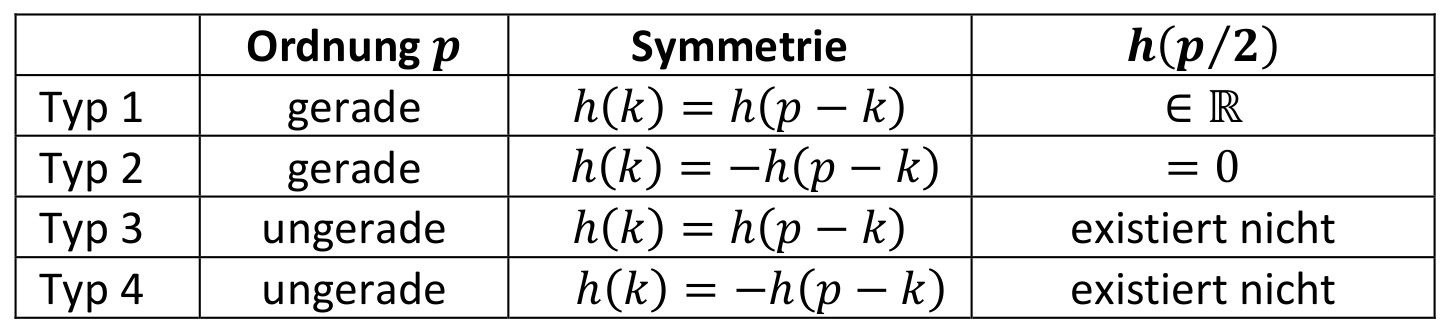
\includegraphics[width=1\textwidth]{./img/Grundtypen_FIR.png}
      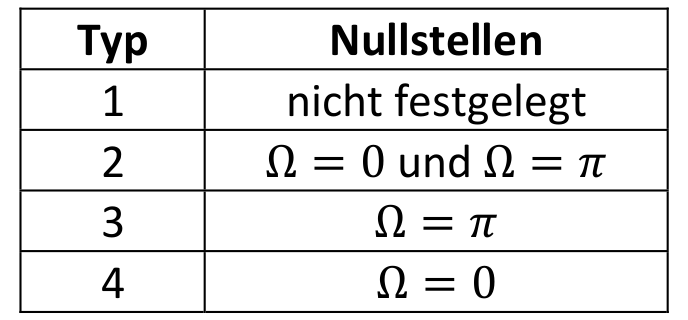
\includegraphics[width=0.5\textwidth]{./img/Grundtypen_FIR_NST.png}
\end{center}
\textbf{Eigenschaften der Typen:}
\begin{itemize}
	\item Typ 1: HP, TP, BP, BSP
	\item Typ 2: kein Hoch- ,Tiefpass \& BSP
	\item Typ 3: kein Hochpass \& BSP
	\item Typ 4: kein Tiefpass \& BSP
\end{itemize}
\end{minipage}
\newpage
%%%%%%%%%%%%%%%%%%%%%%%%%%%%%%%%%%%%% Toleranschema %%%%%%%%%%%%%%%%%%%%%%%%%%%%%%%%%%%%%%%%%%%%%%%%%%%%%%%%
\subsection{Toleranzschema:}

\textbf{Toleranzschema in der log. Notation des \\ \grqq{}filterDesigner\grqq{}: }
  \begin{center}
      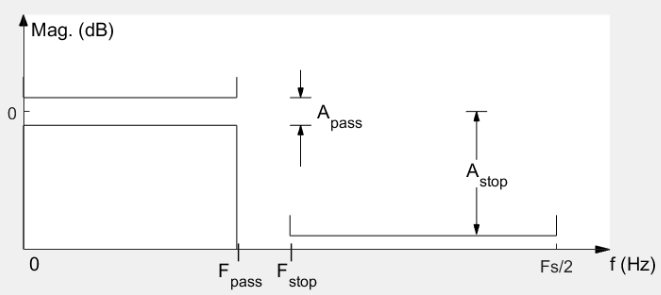
\includegraphics[width=0.5\textwidth]{./img/toleranzschema1.png}
  \end{center}

\textbf{Toleranzschema in der lin. Notation: }
  \begin{center}
    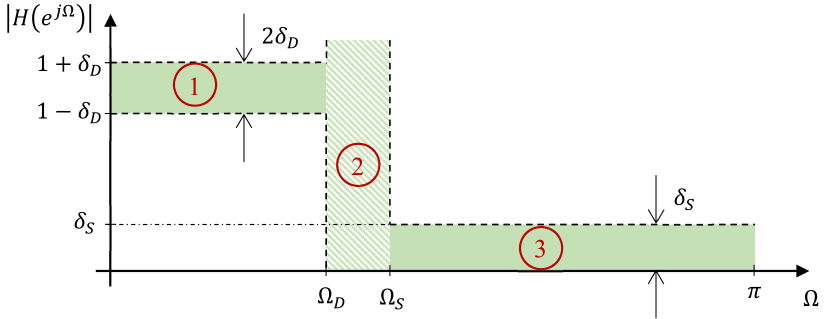
\includegraphics[width=0.5\textwidth]{./img/toleranzschema.png}
  \end{center}
  \begin{mdframed}[style=exercise]
    \begin{align}
      A_{pass}=20~log\left(\textstyle{\frac{1+\delta_{D}}{1-\delta_{D}}}\right)=\abs{20\cdot log_{10}(1-\delta_{D})}\\
      \delta_{D}= 1- 10^{\frac{-A_{pass}}{20}}\\
      A_{Stop}=\abs{20\,log(\delta_{S})}\\
      F_{pass}=\frac{\Omega_{D}}{2\pi}f_{A}\\
      F_{stop}=\frac{\Omega_{S}}{2\pi}f_{A}\\
    \end{align}
  \end{mdframed}
%%%%%%%%%%%%%%%%%%%%%%%%%%%%%%%%%%%%% Kanonische-Formen %%%%%%%%%%%%%%%%%%%%%%%%%%%%%%%%%%%%%%%%%%%%%%%%%%%%%%%%
\subsection{Kanonische Strukturen: }
\begin{itemize}
  \item Realisierung von Filtern mit minimaler Speicherzellenanzahl
  \item für Filter mit Ordnung $p$ sind $p$ Zellen nötig
\subsubsection{1. Kanonische-Form (IIR)}
\end{itemize}
Hälfte der Speicherzellen \& $a_0=1$
  \begin{center}
      \includegraphics[width=.5\textwidth]{./img/kanon1.png}
  \end{center}
\subsubsection{2. Kanonische-Form (IIR)}
  \begin{center}
      \includegraphics[width=.5\textwidth]{./img/kanon2.png}
  \end{center}
\subsubsection{3. Kanonische-Form (IIR)}
\textbf{Kaskadierung} erzeugt dritte karnonische Struktur\\\\
\textbf{ACHTUNG: } \\
Aufteilung in Teilsysteme \textbf{erster} oder \textbf{zweiter} Ordnung\\
 (\grqq{}Second Order Section\grqq{} oder \grqq{}Biquad\grqq{})
  \begin{center}
      \includegraphics[width=.35\textwidth]{./img/kanon3.png}
  \end{center}
  \begin{mdframed}[style=exercise]
    \begin{align}
        H(z)&=\Pi_{\nu=0}^{N_K} H_\nu(z)\\
        H_\nu(z)^{(1)}&=\frac{b_{0\nu}+b_{1\nu}z^{-1}}{1+a_{1\nu}z^{-1}}\\
        H_\nu(z)^{(2)}&=\frac{b_{0\nu}+b_{1\nu}z^{-1}+b_{2\nu}z^{-2}}{1+a_{1\nu}z^{-1}+a_{2\nu}z^{-2}}
    \end{align}
  \end{mdframed}
  \subsubsection{SOS-Faustregel für Biquads (IIR)}
  Aufteilung der Pole-Nullstellen in Biquads, sodass sich Einflüsse auf Frequenzgang ausgleichen.
  Vorgehen:
  \begin{itemize}
      \item Beginnen mit Pol der am dichtesten am EHK liegt
  \end{itemize}
    \begin{center}
        \includegraphics[width=.5\textwidth]{./img/biquad.png}
    \end{center}
\begin{minipage}{0.5\textwidth}   
\subsubsection{4. Kanonische-Form (IIR)}
\textbf{Parallelisierung} durch Partialbruchzerlegung erzeugt vierte karnonische Struktur\\
  \begin{center}
      \includegraphics[width=.5\textwidth]{./img/kanon4.png}
  \end{center}
  \begin{mdframed}[style=exercise]
    \begin{align}
        H(z)=b_0+\sum_{\nu=1}^{N_P}H\nu(z)
    \end{align}
  \end{mdframed}
\end{minipage}
\subsubsection{Trasversalfilter (FIR)}
Kann effizient durch MAC-Befehl realisiert werden. 
Für linearphasige reelwertige FIR-Filter kann die Symmetrie der $b_k$ genutzt werden.
  \begin{center}
      \includegraphics[width=.5\textwidth]{./img/trans.png}
  \end{center}
%%%%%%%%%%%%%%%%%%%%%%%%%%%%%%%%%%%%%%%%%%%%%%%%%%%%%%%%%%%%%%%%%%%%%%%%%%%%%%%%%%%%%%%%%%%%%%%%%%%%%%%%%%
%%%%%%%%%%%%%%%%%%%%%%%%%%%%%%%%%%%%% Abtastung %%%%%%%%%%%%%%%%%%%%%%%%%%%%%%%%%%%%%%%%%%%%%%%%%%%%%%%
\section{Abtastung}
\subsection{Dezimator Ganzzahliges M}
Dezimator = Kompressor 
  \begin{center}
      \includegraphics[width=.35\textwidth]{./img/dezi.png}
  \end{center}
Das Spektrum $X(e^{j\tilde{\Omega}})$ des ursprünglichen Signals x(k) wird um $M$ dezimiert,
was zum Spektrum $X_d(e^{j\Omega})$ führt.
  \begin{mdframed}[style=exercise]
    \begin{align}
        x_d(k)&=x_c(kMT_A)\\
        X(e^{j\tilde{\Omega}})&=\frac{1}{T_A}\sum_{\nu=-\infty}^{\infty} X_c(j\frac{\tilde{\Omega}}{T_A} -\nu\frac{2\pi}{T_A})\\
        X_d(e^{j\Omega})&=\frac{1}{MT_A}\sum_{\mu=-\infty}^{\infty} X_c(e^{j\frac{\Omega}{MT_A} -\mu\frac{2\pi}{MT_A}})\\
        % \tilde{\Omega}&=\frac{\Omega}{M}-i\frac{2\pi}{M}
        X_d(e^{j\Omega})&=\frac{1}{M}\sum_{i=0}^{M-1} X(e^{j\frac{\Omega}{M} -i\frac{2\pi}{M}})\\
    \end{align}
  \end{mdframed}
  \begin{itemize}
    \item Skalierung der Frequenzachse um $\frac{\Omega}{M}$
    \item Verringerung der Periodisierung
    \item Skalierung des Spektrums mit $\frac{1}{M}$
    \item Falls Nyquist-Kriterium $\frac{f_A}{M}>2\tilde{f}_{max}$ nicht erfüllt $\rightarrow$ Hohe Frequenzanteile Tiefpass-Filtern 
  \end{itemize}
  \begin{center}
      \includegraphics[width=.5\textwidth]{./img/dezi2.png}
  \end{center}
%%%%%%%%%%%%%%%%%%%%%%%%%%%%%%%%%%%%%%%%%%%%%%%%%%%%%%%%%%%%%%%%%%%%%%%%%%%%%%%%%%%%%%%%%%%%%%%%%%%%%%%%%%
%%%%%%%%%%%%%%%%%%%%%%%%%%%%%%%%%%%%% Interpolator %%%%%%%%%%%%%%%%%%%%%%%%%%%%%%%%%%%%%%%%%%%%%%%%%%%%%%%
\subsection{Interpolator Ganzzahliges M}
Interpolator = Expander
  \begin{center}
      \includegraphics[width=.4\textwidth]{./img/interpol.png}
  \end{center}
Expander hängt hinter jedem Abtastwert von x(k) L-1 0er an.
$x_e(k)= [x(k/L) \ zeros(1,L-1)]$
  \begin{mdframed}[style=exercise]
    \begin{align}
        x_i(k)&=x_c(k\frac{T_A}{L})\\
        X_e(e^{j\tilde{\Omega}})&=\sum_{\nu=-\infty}^{\infty} x(\nu)e^{-j\Omega\nu L}\\
        X_e(e^{j\Omega}) &=X(e^{j\Omega L})
    \end{align}
  \end{mdframed}
  \begin{itemize}
    \item Spektrum $X_e(e^{j\Omega}) =X(e^{j\Omega L})$ läuft von $-\pi/L ...\pi/L$
    \item Keine Skalierung des Spektrums 
  \end{itemize}
  \begin{center}
      \includegraphics[width=.35\textwidth]{./img/interpol2.png}
  \end{center}
\subsection{Änderung nicht Ganzzahlig}
Zusammenfassung der Tiefpässe zu einem mit V=L und Grenzfrequenz $\Omega_{g,i\&d}=min(\frac{\pi}{L}, \frac{\pi}{M})$
  \begin{mdframed}[style=exercise]
    \begin{align}
        \Omega_{nachher}=\Omega_{vorher}\frac{M}{L}
    \end{align}
  \end{mdframed}

%%%%%%%%%%%%%%%%%%%%%%%%%%%%%%%%%%%%%%%%%%%%%%%%%%%%%%%%%%%%%%%%%%%%%%%%%%%%%%%%%%%%%%%%%%%%%%%%%%%%%%%%%%
%%%%%%%%%%%%%%%%%%%%%%%%%%%%%%%%%%%%%%% Korrespondenztabellen %%%%%%%%%%%%%%%%%%%%%%%%%%%%%%%%%%%%%%%%%%%%
\section{Korrespondenztabellen}
%%%%%%%%%%%%%%%%%%%%%%%%%%%%%%%%%%%%%% Fouriertransformation %%%%%%%%%%%%%%%%%%%%%%%%%%%%%%%%%%%%%%%%%%%%%
%\subsection{Fouriertransformation}
%%%% Rechenregeln
%%%% Quelle: Angepasst nach SDS-Skript
%\begin{center}
%  \bgroup
%  \def\arraystretch{1.5}
%  \begin{tabular}{ | c | c | }
%  \cline{1-2}
%          \rowcolor{black!15}
%          Zeitbereich & Spektralbereich \\
%
%  % Transformation
%  \cline{1-2}
%          $x(t) = \frac{1}{2\pi}\displaystyle\int\limits_{-\infty}^{\infty}X(j\omega)\cdot e^{j\omega{}t}d\omega$ & $X(j\omega) = \displaystyle\int\limits_{-\infty}^{\infty}x(t)\cdot e^{-j\omega{}t}dt$ \\
%
%  % Linearität
%  \cline{1-2}
%          $a\cdot x_1(t)+ b\cdot x_2(t)$ & $a\cdot X_1(j\omega) +b\cdot X_2(j\omega)$ \\
%
%  % Verschiebung
%  \cline{1-2}
%          $x(t-T)$ & $e^{-j\omega{}t} X(j\omega)$\\
%
%  % Dämpfung
%  \cline{1-2}
%          $x(t)\cdot e^{j\omega_{0}t}$ & $X(j\omega-j\omega_0)$\\
%
%  % Differentiation
%  \cline{1-2}
%          $\frac{dx(t)}{dt}$ & $j\omega\cdot X(j\omega)$\\
%
%  % Differentiation (Freq. Bereich)
%  \cline{1-2}
%          $(-jt)^n\cdot x(t)$ & $\frac{d^n}{d\omega^n}X(j\omega)$\\
%          
%  \cline{1-2}
%  \end{tabular}
%  \egroup
%\end{center}

%%%%%%%%%%%%%%%%%%%%%%%%%%%%%%%%% Zeitdiskrete Fouriertransformation %%%%%%%%%%%%%%%%%%%%%%%%%%%%%%%%%%%%%%
\subsection{Zeitdiskrete Fouriertransformation}
%%% Rechenregeln
%%% Quelle: DSV-Skript, Kapitel Elementare DSV
Zeitdiskrete Fouriertransformation ist Grenzwert der DFT für $N\to\infty$ und kann aus der Z-Trafo über $z:=e^{j\Omega}$ gewonnen werden.
\begin{mdframed}[style=exercise]
  \begin{align}
    \Omega=\omega{}T_A=\frac{\omega}{f_A}=2\pi\frac{f}{f_A}
  \end{align}
\end{mdframed}
\begin{center}
  \bgroup
  \def\arraystretch{1.5}
  \begin{tabular}{ | c | c | }
  \cline{1-2}
          \rowcolor{black!15}
          Zeitbereich & Frequenzbereich \\
  
  % Definition
  \cline{1-2}
          \shortstack{$x(k)=$\\ $\frac{1}{2\pi}\displaystyle\int_{-\pi}^{\pi}X(e^{j\Omega})e^{j\Omega{}k}d\Omega$} & $X(e^{j\Omega})=\displaystyle\sum\limits_{k=-\infty}^{\infty}x(k)e^{-j\Omega{}k}$ \\

  % Linearität (angepasst für Klarheit)
  \cline{1-2}
          $a\cdot{}x_1(k)+b\cdot{}x_2(k)$ & $a\cdot{}X_1(e^{j\Omega})+b\cdot{}X_2(e^{j\Omega})$\\

  % Zeitverschiebung
  \cline{1-2}
          $x(k-k_d)$ & $e^{-j\Omega{}k_d}X(e^{j\Omega})$ \\  

  % Frequenzverschiebung
  \cline{1-2}
          $e^{j\Omega_{0}k}x(k)$ & $X(e^{j(\Omega-\Omega_0)})$ \\  

  % Spiegelung 
  \cline{1-2}
          $x(-k)$ & \shortstack{$X(e^{-j\Omega})$\\ $(= X^*(e^{j\Omega}) \text{ für } x(k) \in \mathbb{R})$}\\ 

  % Faltung
  \cline{1-2}
          $x_1(k) * x_2(k)$& $X_1(e^{j\Omega})X_2(e^{j\Omega})$\\ 
  
  % Multiplikation
  \cline{1-2}
          $x_1(k)x_2(k)$ & $\frac{1}{2\pi}\displaystyle\int_{-\pi}^{\pi}X_1(e^{j\Theta})X_2(e^{j(\Omega-\Theta)})d\Theta$ \\  
  \cline{1-2}
  \end{tabular}
  \egroup
\end{center}

%%% Korrespondenzen
\begin{center}
  \bgroup
  \def\arraystretch{1.5}
  \begin{tabular}{ | c | c | }
  \cline{1-2}
          \rowcolor{black!15}
          Zeitbereich & Frequenzbereich \\
  
  % Dirac
  \cline{1-2}
          $\gamma_0(k) \text{ (Dirac)}$ & $1$ \\

  % Sprung
  \cline{1-2}
          $\gamma_{-1}(k) \text{ (Sprung)}$ & $\frac{1}{1-e^{-j\Omega}}+\displaystyle\sum\limits_{\nu=-\infty}^{\infty}\pi\gamma_0(\Omega+2\pi\nu)$\\

  % 1
  \cline{1-2}
          $1$ & $\displaystyle\sum\limits_{\nu=-\infty}^{\infty}2\pi\gamma_0(\Omega+2\pi\nu)$ \\  

  % Verschobener Dirac
  \cline{1-2}
          $\gamma_0(k-k_0)$ & $e^{-j\Omega{}k_0}$ \\  

  % Exponentialfunktion 
  \cline{1-2}
          $a^{k}\gamma_{-1}(k)\:(|a|<1)$ & $\frac{1}{1-ae^{-j\Omega}}$\\ 

  % si-Like
  \cline{1-2}
          $\frac{\sin(\Omega_{c}k)}{\pi{}k}$& $X(e^{j\Omega}) =
          \begin{cases}
              1,\:|\Omega|<\Omega_c \\
              0,\:\Omega_c < |\Omega| \leq \pi
          \end{cases}
          $\\ 
  
  % rect (Verschoben)
  \cline{1-2}
          $x(k)=
          \begin{cases}
            1,\:0\leq{}k\leq{}M \\
            0,\:sonst
          \end{cases}$ & $\frac{\sin(\Omega(M+1)/2)}{\sin(\Omega/2)}e^{-j\Omega{}\frac{M}{2}}$ \\  
  
  % cos
  \cline{1-2}
          $\cos(\Omega_{0}k+\varphi)$ & \shortstack{$\displaystyle\sum\limits_{\nu=-\infty}^{\infty} [\pi{}e^{j\varphi}\gamma_0(\Omega-\Omega_0+2\pi\nu)$ \\ $+\pi{}e^{-j\varphi}\gamma_0(\Omega+\Omega_0+2\pi\nu)]$} \\
  \cline{1-2}
  \end{tabular}
  \egroup
\end{center}
%%%%%%%%%%%%%%%%%%%%%%%%%%%%%%%%% Diskrete Fouriertransformation %%%%%%%%%%%%%%%%%%%%%%%%%%%%%%%%%%%%%%
\begin{minipage}{0.5\textwidth}  
\subsection{DFT}
DFT nimmt implizit unendlich periodische Fortsetzung des Signals an. Zu beachten: $-1_{modN}=-1 + N$, $-2_{modN}=-2+N$, ... (solange Addition von N bis positiv!).\\
\textbf{Math. Modulo:}
$\tilde{x}(k) = x([k]_{modN})$ 
$[n]_{modN}=n-N \lfloor \frac{n}{N} \rfloor$
  \begin{center}
      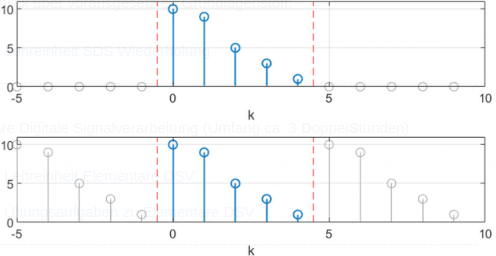
\includegraphics[width=1\textwidth]{./img/x_k.png}
      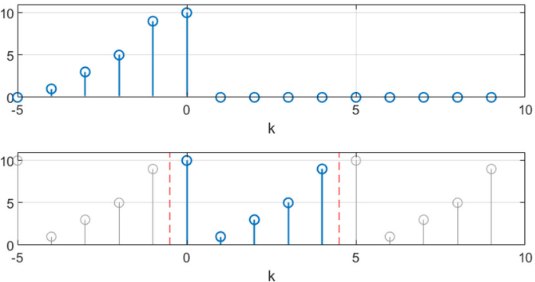
\includegraphics[width=1\textwidth]{./img/x_mk.png}
  \end{center}

%%% Rechenregeln
%%% Quelle: DSV-Skript, Kapitel Elementare DSV
\begin{center}
  \bgroup
  \def\arraystretch{1.5}
  \begin{tabular}{ | c | c | }
  \cline{1-2}
          \rowcolor{black!15}
          Zeitbereich & Frequenzbereich \\
  
  % Definition
  \cline{1-2}
          \shortstack{$x(k)=\text{IDFT}_N\{X(n)\}$ \\ $=\frac{1}{N}\displaystyle\sum\limits_{n=0}^{N-1}X(n)e^{j\frac{2\pi}{N}kn}$} &
          \shortstack{$X(n)=\text{DFT}_N\{x(k)\}$ \\ $=\displaystyle\sum\limits_{k=0}^{N-1}x(k)e^{-j\frac{2\pi}{N}kn}$} \\

  \cline{1-2}
          $a\cdot x_1(k)+ b\cdot x_2(k)$ & $a\cdot X_1(n) +b\cdot X_2(n)$ \\
  \cline{1-2}
          $x([k\textcolor{red}{-}k_0]_{modN})$ & $e^{\textcolor{red}{-}j\frac{2\pi nk_0}{N}} X(n)$\\
  \cline{1-2}
          $e^{\textcolor{red}{-}j\frac{2\pi nk_0}{N}} x(k)$ & $X([n\textcolor{red}{+}k_0]_{modN})$ \\  
  \cline{1-2}
          $x([-k]_{modN})$ & $X([-n]_{modN})$ \\  
  \cline{1-2}
          $x^*(k)$& $X^*([-n]_{modN})$\\ 
  \cline{1-2}
          $x^*([-k]_{modN})$& $X^*(n)$\\ 
  \cline{1-2}
          $x_1(k) \circledast x_2(k)$ & $X_1(n)X_2(n)$ \\  
  \cline{1-2}
          $x_1(k)x_2(k)$ & $\frac{1}{N} X_1(n) \circledast X_2(n)$ \\
  \cline{1-2}
          $x_g(k)=\frac{x(k)+\tilde{x}(-k)}{2}$ & $X_g(n)=\frac{X(n)+X(-n)}{2}$ \\
  \cline{1-2}
          $x_u(k)=\frac{x(k)-\tilde{x}(-k)}{2}$ & $X_u(n)=\frac{X(n)-X(-n)}{2j}$ \\
  \cline{1-2}
  \end{tabular}
  \egroup
\end{center}
\end{minipage}
%%%%%%%%%%%%%%%%%%%%%%%%%%%%%%%%%% Z-Transformation (einseitig) %%%%%%%%%%%%%%%%%%%%%%%%%%%%%%%%%%%%%%%%%%%
\begin{minipage}{0.5\textwidth}  
\subsection{Z-Transformation (einseitig)}
%%% Regeln
%%% Quelle: DSV-Skript, Kapitel Elementare DSV
\begin{mdframed}[style=exercise]
  \begin{align}
    x(0) &= \lim_{z\to\infty}X(z) \\
    \lim_{k\to\infty}x(k) &= \lim_{z\to1+}(z-1)X(z)
  \end{align}
\end{mdframed}
\begin{center}
  \bgroup
  \def\arraystretch{1.5}
  \begin{tabular}{ | c | c | }
  \cline{1-2}
          \rowcolor{black!15}
          Zeitbereich & Z-Bereich \\
  
  % Definition
  \cline{1-2}
          $x(k)=\frac{1}{2\pi{}j}\displaystyle\oint_{C}X(z)z^{k-1}dz$ &
          $X(z)=\displaystyle\sum\limits_{k=0}^{\infty}x(k)z^{-k}$ \\

  % Linearität
  \cline{1-2}
          $a\cdot x_1(k)+ b\cdot x_2(k)$ & $a\cdot X_1(z) +b\cdot X_2(z)$ \\

  % Verschiebung (negativ)
  \cline{1-2}
          $x(k-i)$ & $z^{-i}\cdot{}X(z)$\\

  % Verschiebung (positiv)
  \cline{1-2}
        $x(k+i)$ & \shortstack{$z^i\cdot{}X(z)-\displaystyle\sum\limits_{\mu=0}^{i-i}z^{i-\mu}x(\mu)$ \\ 
        \text{(meistens $z^i\cdot{}X(z)$)}}\\

  % Faltung
  \cline{1-2}
          $x_1(k) * x_2(k)$ & $X_1(z)X_2(z)$ \\ 
  
  % Summation
  \cline{1-2}
          $\displaystyle\sum\limits_{\mu=0}^{k}x(\mu)$ & $\frac{z}{z-1}X(z)$ \\  
  
  % Modulation
  \cline{1-2}
          $z_0^{k}x(k)$ & $X(\frac{z}{z_0})$ \\ 

  % Multiplikation
  \cline{1-2}
          $x_1(k)x_2(k)$ & $\frac{1}{2\pi}\displaystyle\oint_{C}X_1(w)X_2(\frac{z}{w})w^{-1}dw$\\ 

  % Multiplikation (Spezialfall 1)
  \cline{1-2}
          $kx(k)$ & $-z\frac{d}{dz}X(z)$ \\  

  % Multiplikation (Spezialfall 2)
  \cline{1-2}
          $k^{2}x(k)$ & $z^{2}\frac{d^2}{dz^2}X(z)+z\frac{d}{dz}X(z)$ \\
  
  % Konjugiert komplex
  \cline{1-2}
          $x^*(k)$ & $X^*(z^*)$ \\
  \cline{1-2}
  \end{tabular}
  \egroup
\end{center}
\end{minipage}

%%% Korrespondenzen
\textbf{Alle $x(k)=0$ für $k < 0$}.
\begin{center}
  \bgroup
  \def\arraystretch{1.5}
  \begin{tabular}{ | c | c | }
  \cline{1-2}
          \rowcolor{black!15}
          Zeitbereich & Z-Bereich \\
  
  \cline{1-2}
          $\gamma_0(k)$ &
          $1$ \\

  \cline{1-2}
          $z_0^k$ & $\frac{z}{z-z_0}$ \\

  \cline{1-2}
          $\gamma_{-1}(k)$ & $\frac{z}{z-1}$\\

  \cline{1-2}
        $\cos(\Omega_0k+\varphi)$ & $\frac{z(z\cos(\varphi)-cos(\Omega_0+\varphi))}{z^2-2z\cos(\Omega_0)+1}$ \\ 

  \cline{1-2}
          $\cos(\Omega_0k)$ & $\frac{z(z-\cos(\Omega_0))}{z^2-2z\cos(\Omega_0)+1}$ \\ 
  
  \cline{1-2}
          $\sin(\Omega_0k)$ & $\frac{z\sin(\Omega_0)}{z^2-2z\cos(\Omega_0)+1}$ \\  
  
  \cline{1-2}
          $k$ & $\frac{z}{(z-1)^2}$ \\ 

  \cline{1-2}
          $kz_0^k$ & $\frac{zz_0}{(z-z_0)^2}$\\ 

  \cline{1-2}
          $k^2z_0^k$ & $\frac{zz_0(z+z_0)}{(z-z_0)^3}$ \\  

  \cline{1-2}
          \shortstack{$\binom{k}{n}=\frac{k!}{(k-n)!n!}$ \\ $(=0, \forall{}k<n)$} & $\frac{z}{(z-1)^{n+1}}$ \\
  
  \cline{1-2}
  \end{tabular}
  \egroup
\end{center}
 \newpage
%%%%%%%%%%%%%%%%%%%%%%%%%%%%%%%%%%%%%%%%%%%%%%%%%%%%%%%%%%%%%%%%%%%%%%%%%%%%%%%%%%%%%%%%%%%%%%%%%%%%%%%%%%
%%%%%%%%%%%%%%%%%%%%%%%%%%%%%%%%%%%%% Mathe-Tricks %%%%%%%%%%%%%%%%%%%%%%%%%%%%%%%%%%%%%%%%%%%%%%%%%%%%%%% 
\section{Mathematische Anmerkungen}
\begin{mdframed}[style=exercise]
    \begin{align}
     \textbf{Eueler Formel: } e^{i\Omega} = cos(\Omega) + i\cdot sin(\Omega)\\
     cos(\Omega) = \frac{e^{-i\Omega}+e^{+i\Omega}}{2}\\
     sin(\Omega) = \frac{e^{-i\Omega}-e^{-i\Omega}}{2j}\\
     cos(\pi\cdot k) = (-1)^{k}\\
     cos^{2}(k)+sin^{2}(k)=1\\
    \textbf{Rechteck-Funktion: } rect(\frac{t-t_{0}}{T})
    \end{align}
\end{mdframed}

\subsection{Dezibel-Umrechnung}
\begin{itemize}
	\item \textbf{lin-dB-Rechnung: }$[db]=a\cdot 10\cdot \log_{10}[lin]$
    	\item \textbf{dB-lin-Rechnung: }$[lin]=10^{\frac{[dB]}{a}}$
    	\item \textbf{Vorfaktor: } Feldgröße: $a=20$ Energiegröße: $a=10$
\end{itemize}

\subsection{Komplexe Zahlen}
\begin{mdframed}[style=exercise]
    \begin{align}
    \textbf{Komplexer Betrag: } \abs{x} = \sqrt{Re^{2}+Im^{2}}\\
    \textbf{Phase: } \varphi = arctan(\frac{\grqq{}Imag.\grqq{}}{\grqq{}Real.\grqq{}})=arctan(\frac{sin(\varphi)}{cos(\varphi)})\\
    arg(\frac{a(j\Omega)\cdot b(j\Omega)}{c(j\Omega)})=arg(a)+arg(b)-arg(c)
    \end{align}
\end{mdframed}

\textbf{Phasenkorrektur bei $\varphi=arg(x+j\cdot y)$: }
\begin{itemize}
	\item $arctan(\frac{y}{x})$ für $x > 0$ 
	\item $arctan(\frac{y}{x}) + \pi$ für $x < 0$ $y \geq 0$ 
	\item $arctan(\frac{y}{x}) - \pi$ für $x < 0$ $y < 0$ 
	\item $\frac{\pi}{2}$ für $x = 0$ $y > 0$
	\item $\frac{-\pi}{2}$ für $x = 0$ $y < 0$
	\item unbestimmt für $x = 0$ $y = 0$
\end{itemize}

\begin{mdframed}[style=exercise]
    \begin{align}
     sin(\frac{2\cdot\pi\cdot f_{sin}\cdot k}{f_{A}}) = \frac{1}{2j}\cdot (e^{\frac{j\cdot 2\cdot\pi\cdot f_{sin}\cdot k}{f_{A}}}-e^{\frac{j\cdot 2\cdot\pi\cdot f_{sin}\cdot k}{f_{A}}})
    \end{align}
\end{mdframed}
\newpage
%%%%%%%%%%%%%%%%%%%%%%%%%%%%%%%%%%%%%%%%%%%%%%%%%%%%%%%%%%%%%%%%%%%%%%%%%%%%%%%%%%%%%%%%%%%%%%%%%%%%%%%%%%
%%%%%%%%%%%%%%%%%%%%%%%%%%%%%%%%%%%%% Rechteck als Fensterfunktion%%%%%%%%%%%%%%%%%%%%%%%%%%%%%%%%%%%%%%%%% 
\subsection{Rechteck als Fensterfunktion}
\begin{itemize}
    \item Betragsgang variiert periodisch nach si-Funktion
    \item Breite der Hauptkeule: $\frac{2}{T}$ bzw. $\frac{4\pi}{T}$ (auf $2\pi$ bezogen)
    \item Breite der Nebenkeulen: $\frac{1}{T}$ bzw. $\frac{2\pi}{T}$ (auf $2\pi$ bezogen)
    \item \textbf{T:} Breite des Rechtecks
  \end{itemize}
\begin{mdframed}[style=exercise]
    \begin{align}
\abs{F\{rect(\dfrac{t-T/2}{T})\}} = \abs{T \cdot \dfrac{sin(\Omega\cdot T/2)}{\Omega\cdot T/2}}\\
= \abs{T \cdot si(\Omega\cdot\frac{T}{2})\cdot e^{-j\Omega\cdot T / 2}}
    \end{align}
\end{mdframed}

\begin{center}
      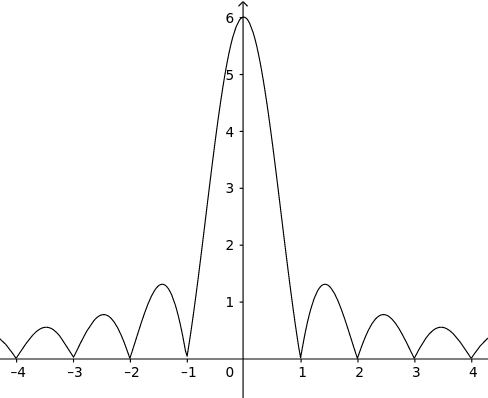
\includegraphics[width=0.4\textwidth]{./img/si_funktion.png}
 \end{center}
 \newpageS
 %%%%%%%%%%%%%%%%%%%%%%%%%%%%%%%%%%%%%%%%%%%%%%%%%%%%%%%%%%%%%%%%%%%%%%%%%%%%%%%%%%%%%%%%%%%%%%%%%%%%%%%%%%
%%%%%%%%%%%%%%%%%%%%%%%%%%%%%%%%%%%%% Hinweise Diagramme %%%%%%%%%%%%%%%%%%%%%%%%%%%%%%%%%%%%%%%%%%%%%%%%%%
\begin{minipage}{0.5\textwidth} 
\section{Interpretation von Diagrammen}
\subsection{Spektrogram:}
\begin{itemize}
    \item Spektrogram zeigt Frequenzanteile gemäß FFT/DFT
    \item Höchste Frequenz entspricht Abtastfrequenz
\end{itemize}

\subsection{Periodogram:}  
\begin{itemize}
    \item Periodogram zeigt Schätzung des Autoleistungsdichte-Spektrums 
    \item Gewichtetes Betragsquadrat des Amplitudenspektrums
    \item $\hat{\phi}_{Per} = \frac{1}{N}\abs{X(n)}^2$
\end{itemize}  

\subsection{Bedeutung der Diagramm-Werte im Bezug auf ein Beispiel-Signal}
$x[k] = a\cdot cos(\Omega_{0}\cdot k)$
\begin{itemize}
    \item Spektrog.: $max(\abs{X[\Omega]})= a\cdot\frac{N}{2}$ 
    \item Periodog.: $max(\hat{\phi}_{Per})= a^{2}\cdot\frac{N}{4}$ 
\end{itemize}
\end{minipage}
\newpage
%%%%%%%%%%%%%%%%%%%%%%%%%%%%%%%%%%%%%%%%%%%%%%%%%%%%%%%%%%%%%%%%%%%%%%%%%%%%%%%%%%%%%%%%%%%%%%%%%%%%%%%%%%
%%%%%%%%%%%%%%%%%%%%%%%%%%%%%%%%%%%%% Taschenrechner-Tricks %%%%%%%%%%%%%%%%%%%%%%%%%%%%%%%%%%%%%%%%%%%%%%%

\section{Taschenrechner-Tricks (fx-991DEX)}
\begin{itemize}
    \item \textbf{Polstellen-Bestimmung:}  
   	 \begin{enumerate}
    	 \item \grqq{}MENU SETUP\grqq{}
    	 \item $({X \atop =}{Y \atop 0})$ \grqq{}A:Gleichung/Funkt\grqq{}
    	 \item \grqq{}=\grqq{}
    	 \item \grqq{}2:Polynom-Gleichung\grqq{}
    	 \end{enumerate}
	 \textbf{ACHTUNG:} Grad muss $\leq 4$ UND $\geq 1$ sein!
     \item \textbf{Leckeffekt-Erkennung \& Behebung:}
     	 \begin{enumerate}
     	 \item $\frac{f_{Abtast}}{f_{Signal}}(=N_{Signal})$ in Taschenrechner eingeben\\
     	 $N_{Signal}$: Anzahl der Abtastwerte in einzelner Periode des Signales
     	 \item Ergebnis \textbf{ganzzahlig} -> kein Leckeffekt
     	 \item Ergebnis in \textbf{Bruch-Form} -> Leckeffekt
     	 \item WENN Bruch: $\frac{N_{Abtast}}{n_{Ganzzahl}}=N_{Signal}$\\
     	 \textbf{$N_{Abtast}$: } kleinste Anzahl an Abtastwerten ohne Leckeffekt\\
     	 \textbf{$n_{Ganzzahl}$: } Ganzzahliges Vielfaches
         \end{enumerate}	 	 
\end{itemize}

\end{document}
